\section{The amplitude fitting results}
\label{chap:Amplitude}

\subsection{{Fit with $N^*$ only}}
%We first show that by including all the $N^*$ in Table~\ref{tab:Lstar} labelled as extended model (\EM),
Firstly,
all the $N^{*}$ are included in the fitting model,
the fit still can't describe the data in some region. 
In Figure.~\ref{fig:Pc-fit-noz}, 
the fit results are presented. 
The data is reasonably reproduced by the fit except for the region with $m_{\proton\pi}>1.8$\gev. 
To check this region the projections of $m_{\jpsi p}$ and $m_{\jpsi \pi}$ are shown in three slices: 
$m_{p\pi}<1.45$\gev,  $1.45<m_{p\pi}<1.80$\gev, and  $m_{p\pi}>1.80$\gev, 
in Figure.~\ref{noZ-mjpsip-bins} and~\ref{noZ-mjpsipi-bins}, respectively. 
The $m_{\jpsi\proton}$ projection in the largest $m_{\proton\pi}$ region shows some evidence of 
the recently observed $\ZP$ states~\supercite{LHCb-PAPER-2019-014}.  
While the $m_{\jpsi\pi}$ projection in the same $m_{\jpsi\pi}$ region shows small excess between 4.0 to 4.4\gev, 
which is the region of the broad $Z_c(4200)$ state, 
observed by the Belle collaboration~\supercite{Chilikin:2014bkk}. 
In the next section, 
each of their possible contributions are checked.


\begin{figure}[!tb]
\centering
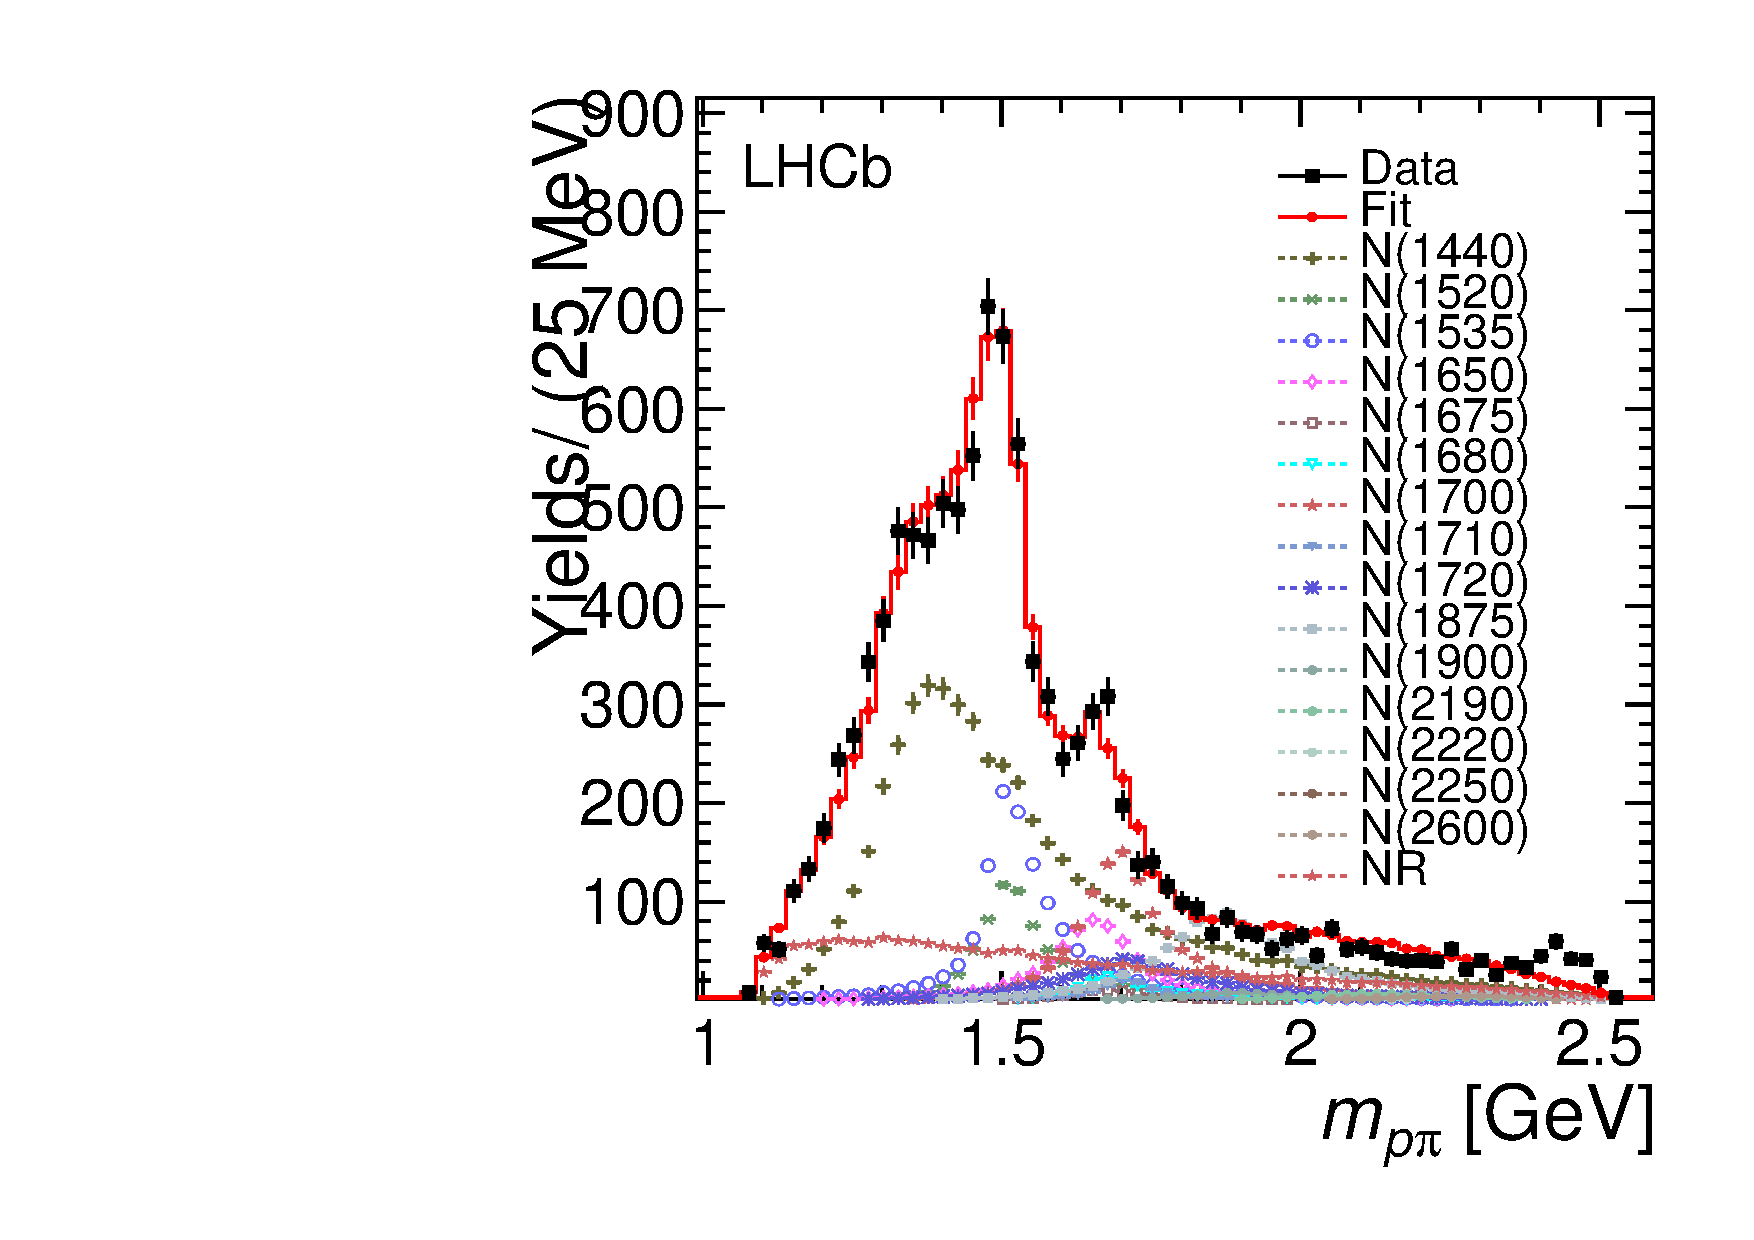
\includegraphics[width=0.4\textwidth]{Figures/04_Penta/05_fit_result/no_pc_plots/mppi_S}%
\put(-150,140) {\textrm{\small \bf Unofficial}}
   \vskip -0.5cm
   \caption{Fit projections for $m_{\proton\pi}$ with $N^{*}$ resonances. 
   The data are shown as solid (black) squares, 
   while the solid (red) line show the results of the fit.  
   The background is subtracted by sPlot technique. 
   Each $N^*$ component is also shown. 
   The error bars on the points showing the fit results are due to simulation statistics.}
   \label{fig:Pc-fit-noz}
\end{figure}


\begin{figure}[!tbh]
\begin{center}
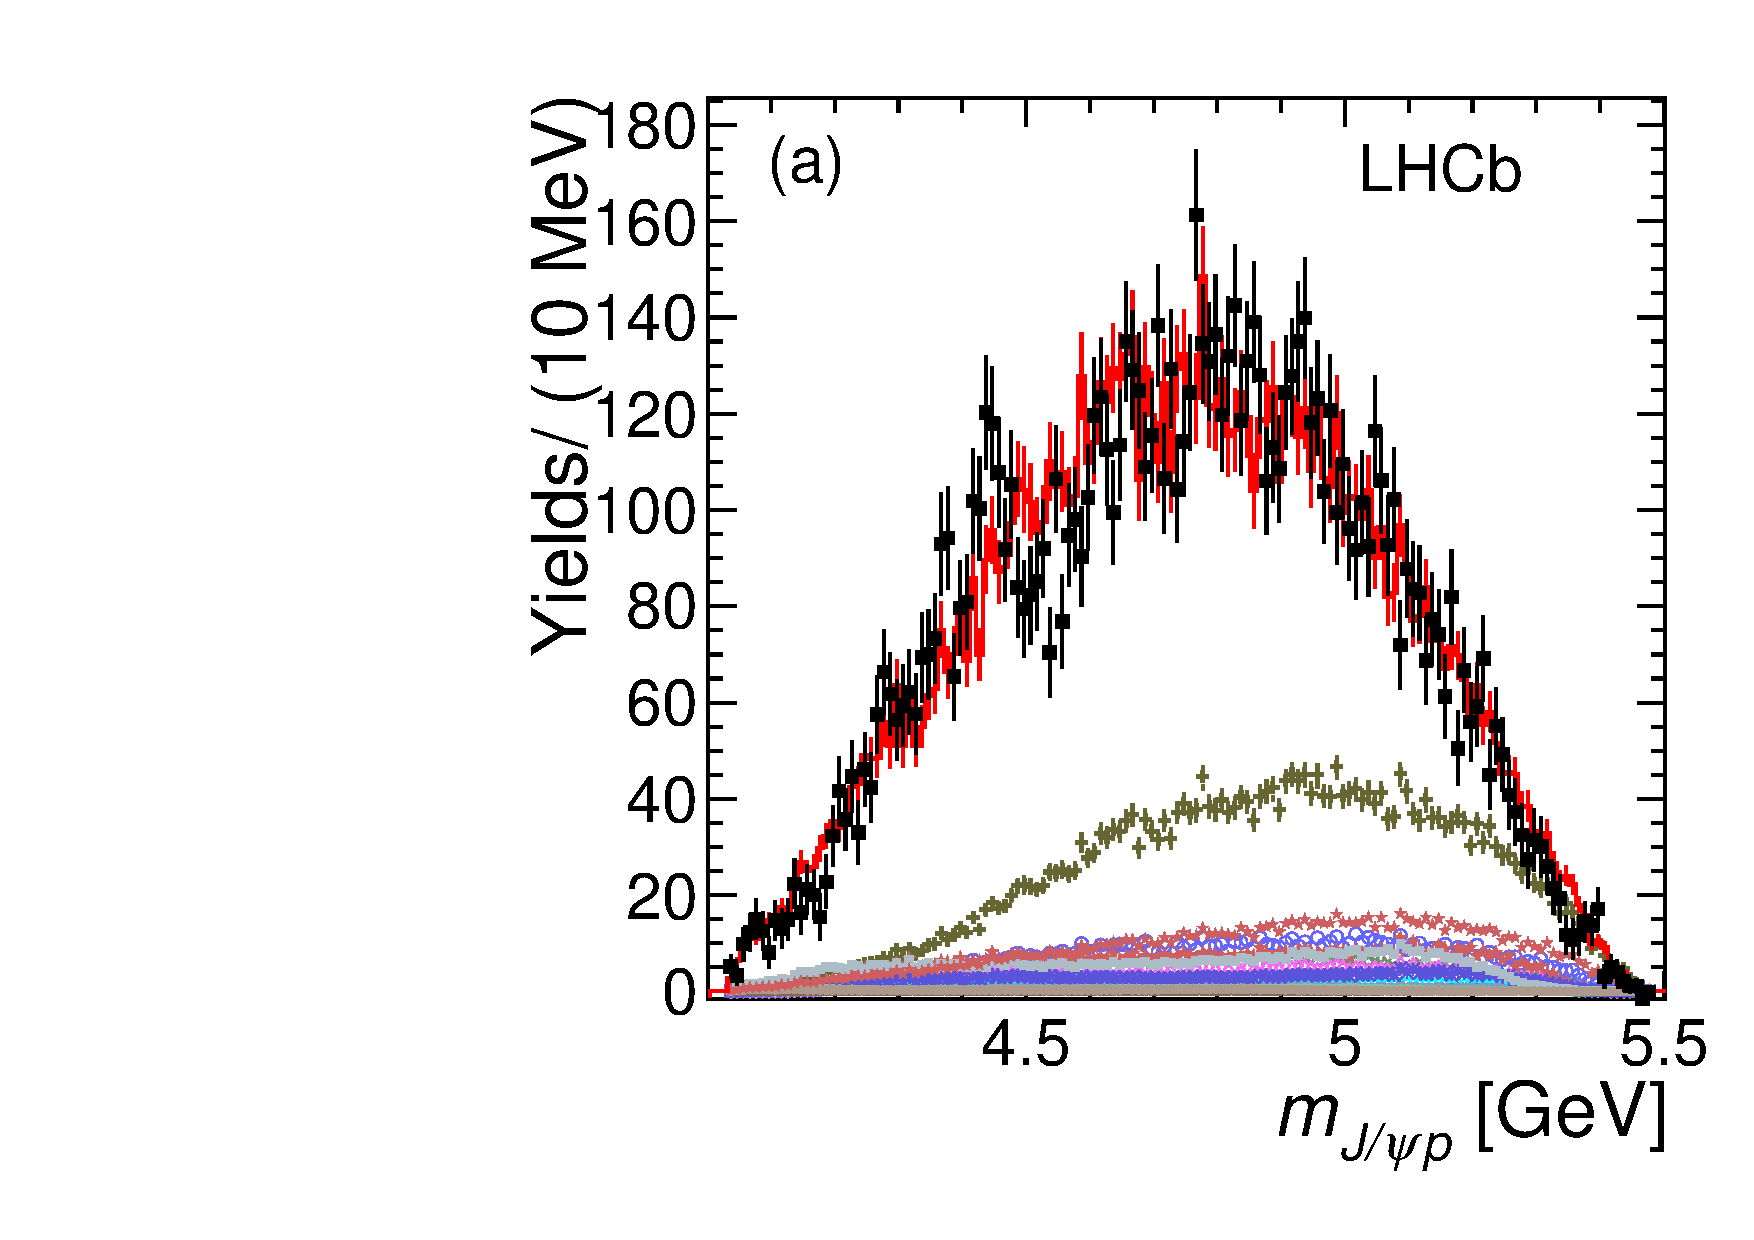
\includegraphics[width=0.4\textwidth]{Figures/04_Penta/05_fit_result/no_pc_plots/mjpsip0}%
\put(-60,140) {\textrm{\small \bf Unofficial}}
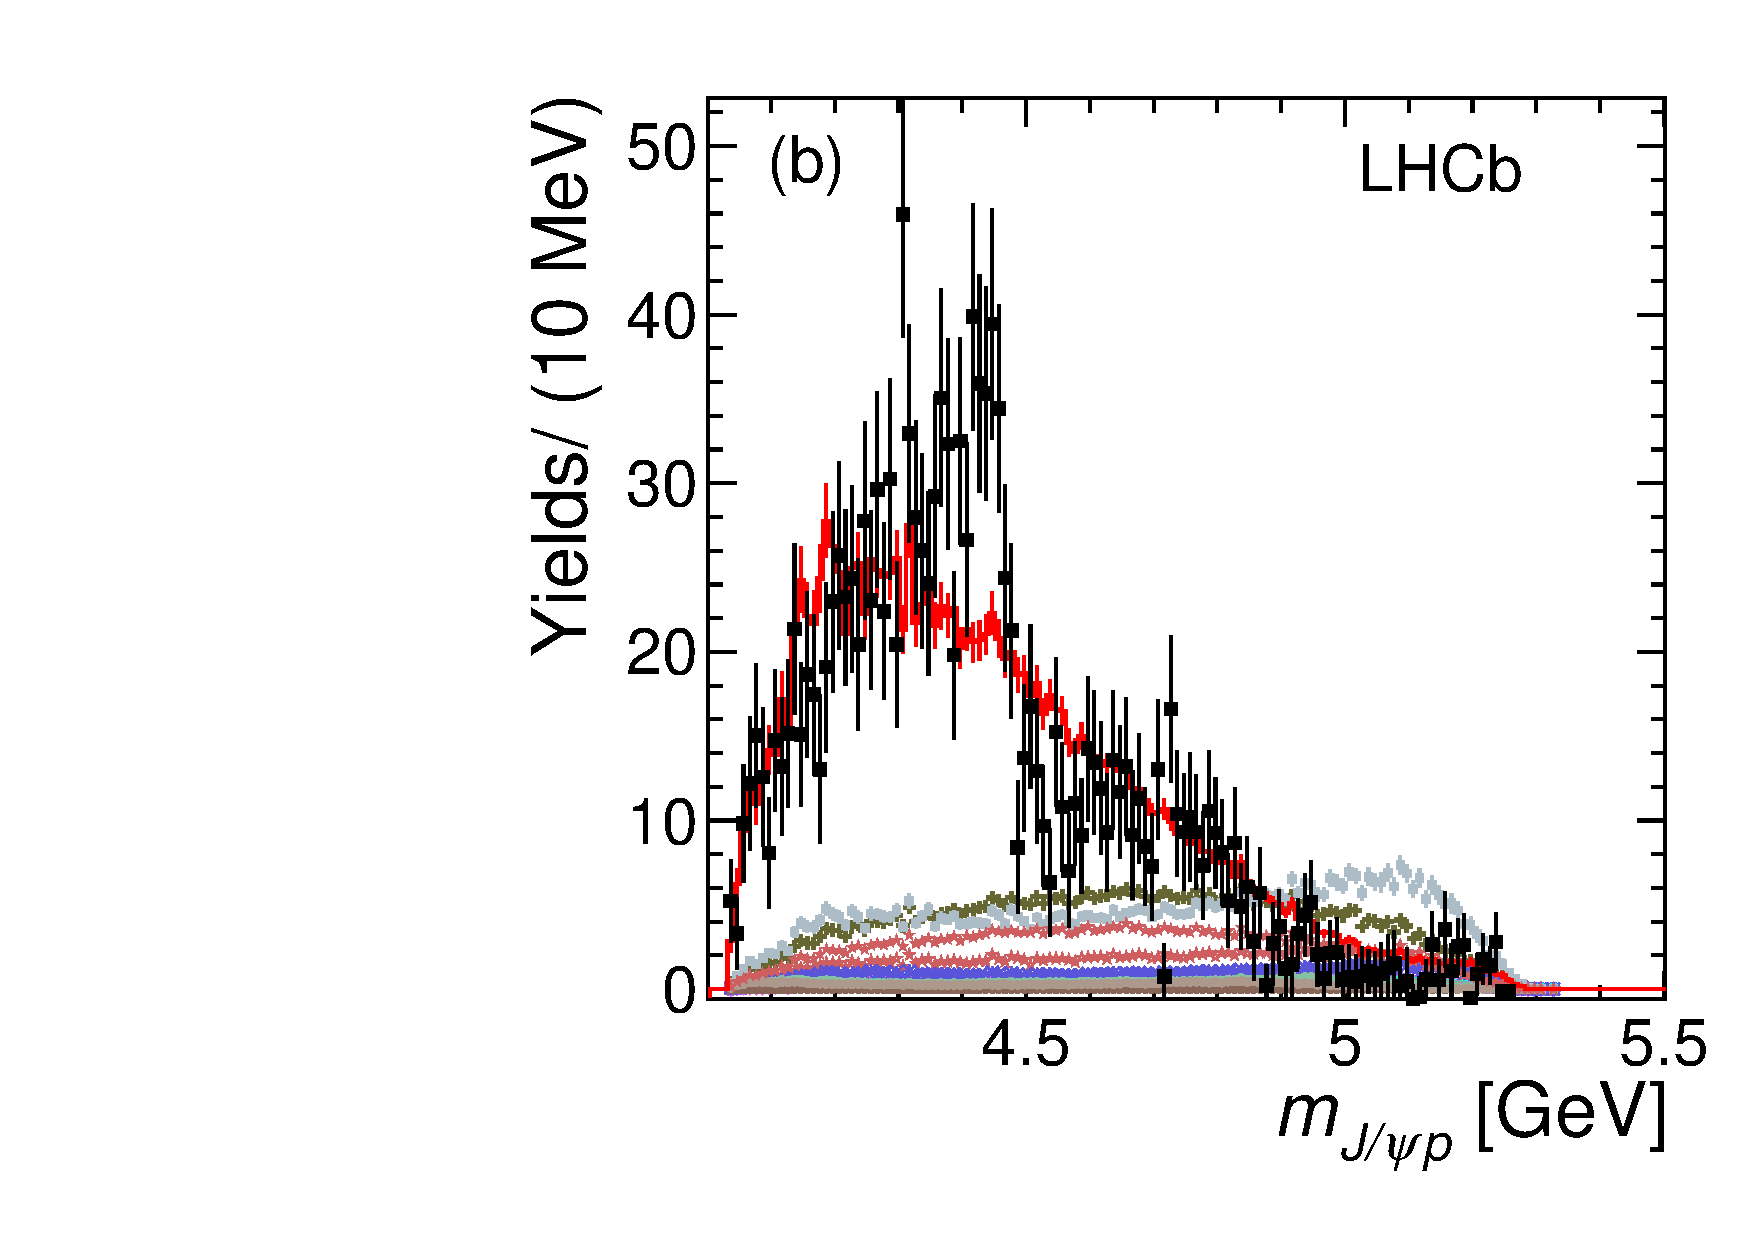
\includegraphics[width=0.4\textwidth]{Figures/04_Penta/05_fit_result/no_pc_plots/mjpsip3}
\put(-60,140) {\textrm{\small \bf Unofficial}} \\
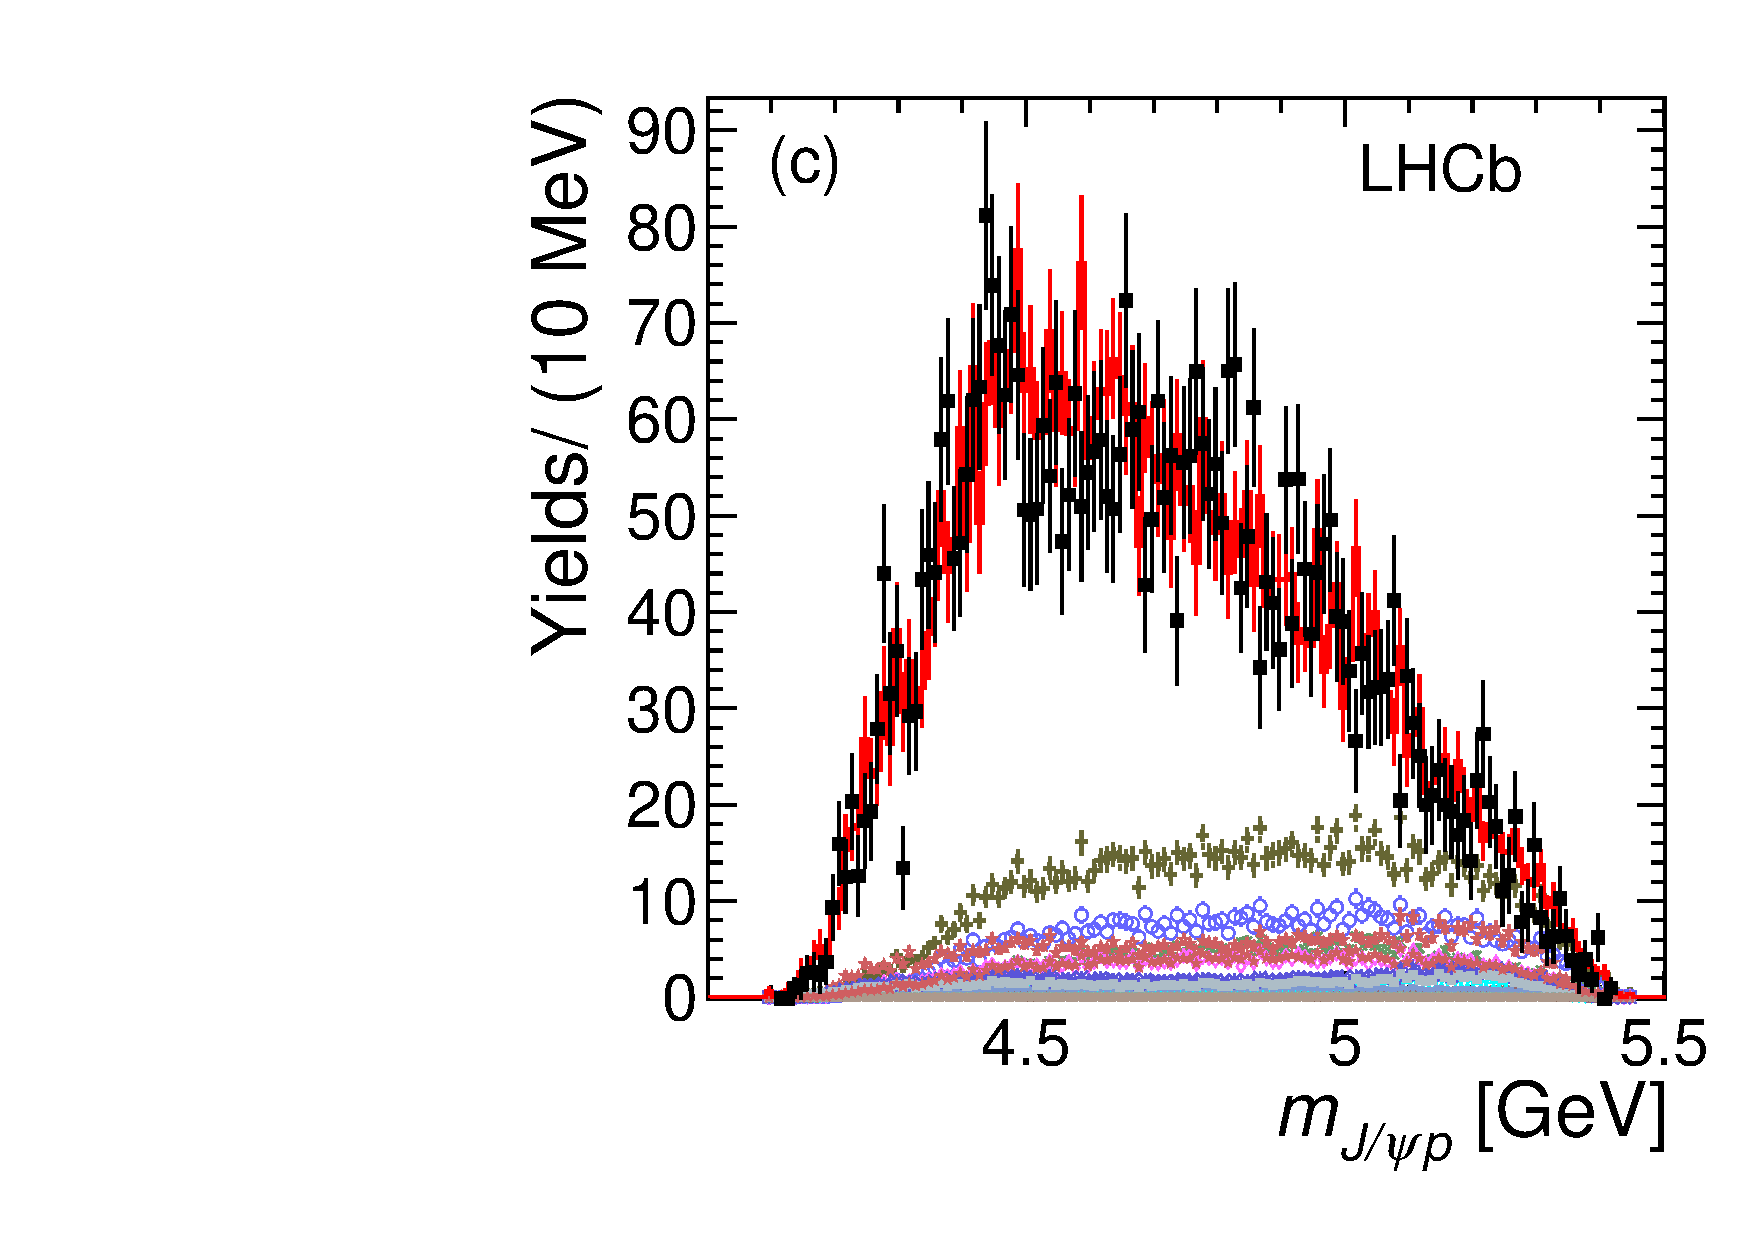
\includegraphics[width=0.4\textwidth]{Figures/04_Penta/05_fit_result/no_pc_plots/mjpsip2}
\put(-60,140) {\textrm{\small \bf Unofficial}}
\end{center}
\vskip -0.5cm
   \caption{$m_{\jpsi \proton}$ in various intervals of $m_{\proton\pi}$ with $N^{*}$ resonances: 
   (a) no $m_{p\pi}$\gev cut, (b) $m_{p\pi}>1.80$\gev, and (c) $1.45<m_{p\pi}<1.80$\gev. 
   The data are shown as (black) squares, while the (red) lines show the results of the fit.} 
\label{noZ-mjpsip-bins}
\end{figure}


\begin{figure}[!tbh]
\begin{center}
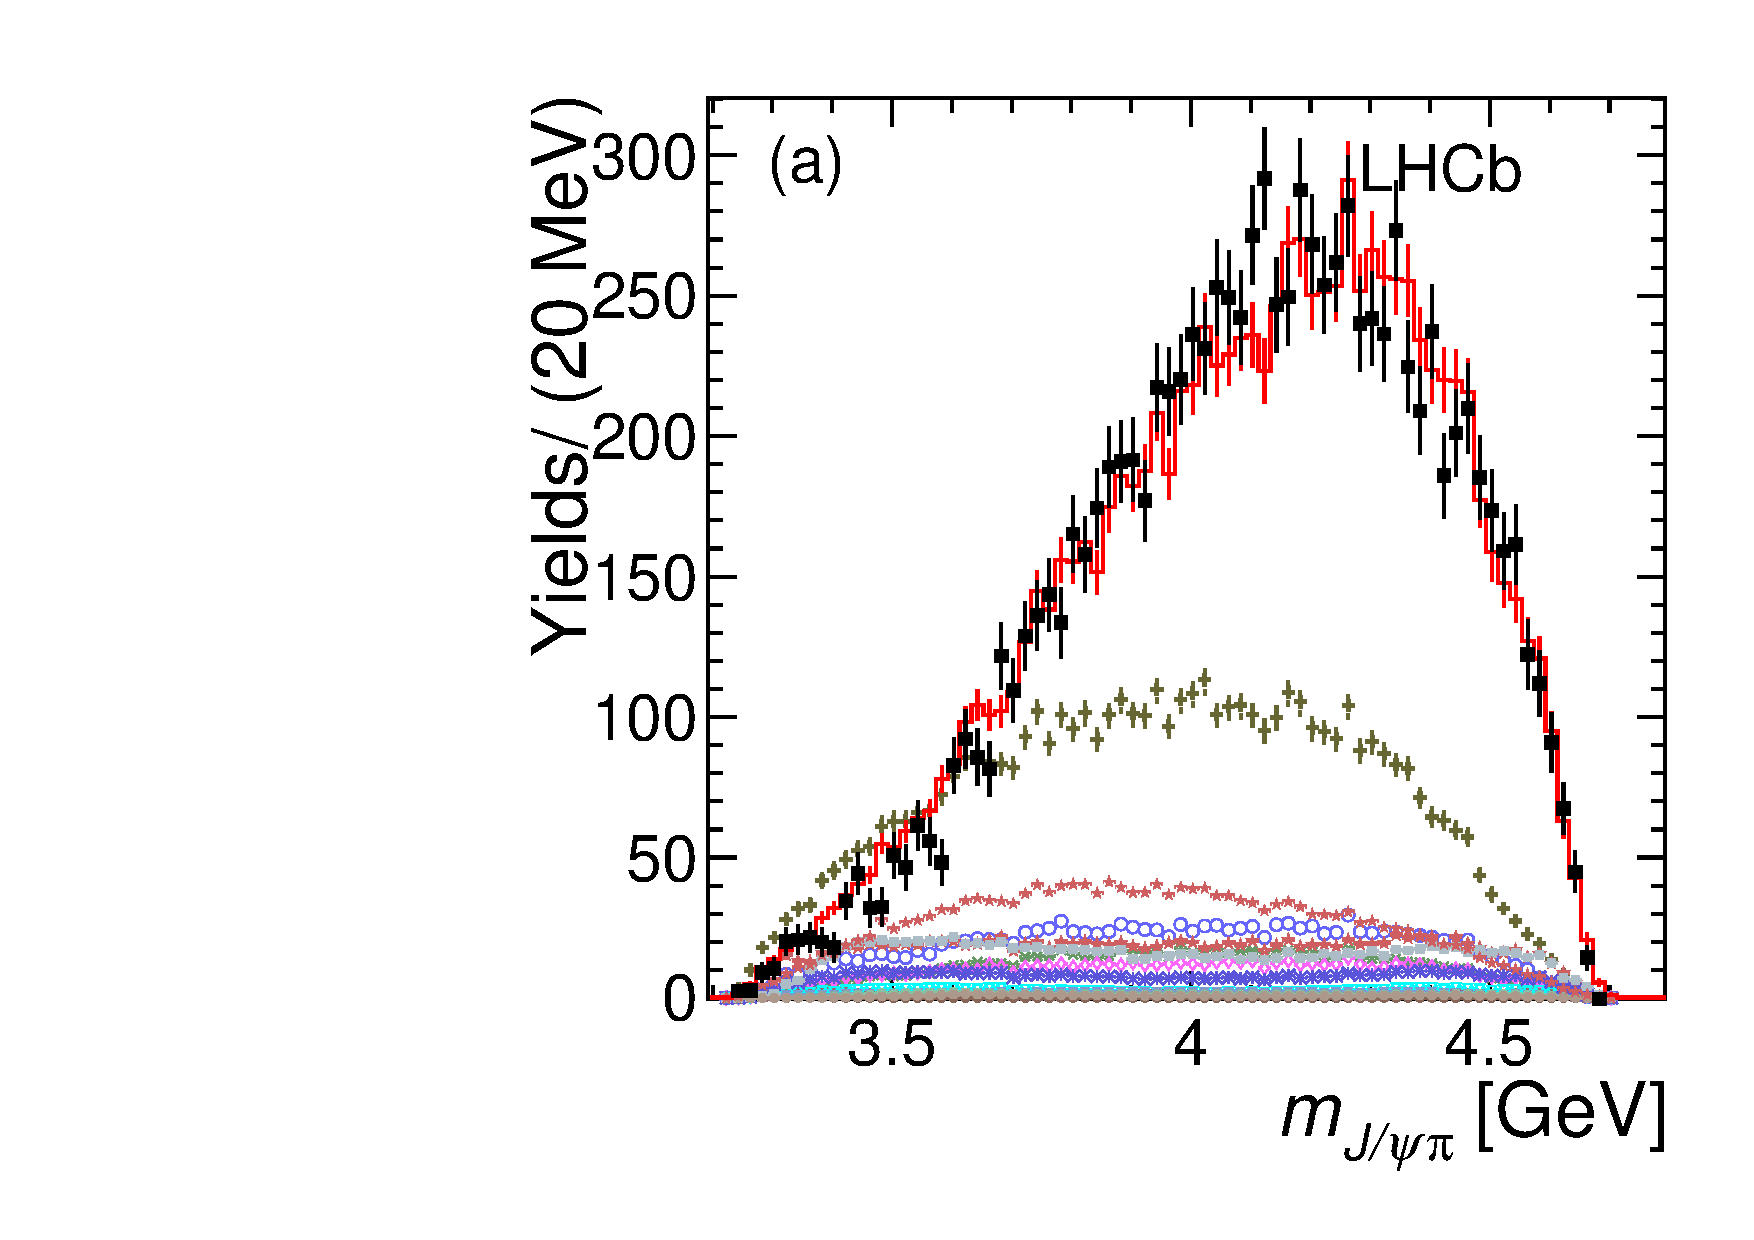
\includegraphics[width=0.4\textwidth]{Figures/04_Penta/05_fit_result/no_pc_plots/mjpsik0}%
\put(-150,140) {\textrm{\small \bf Unofficial}}
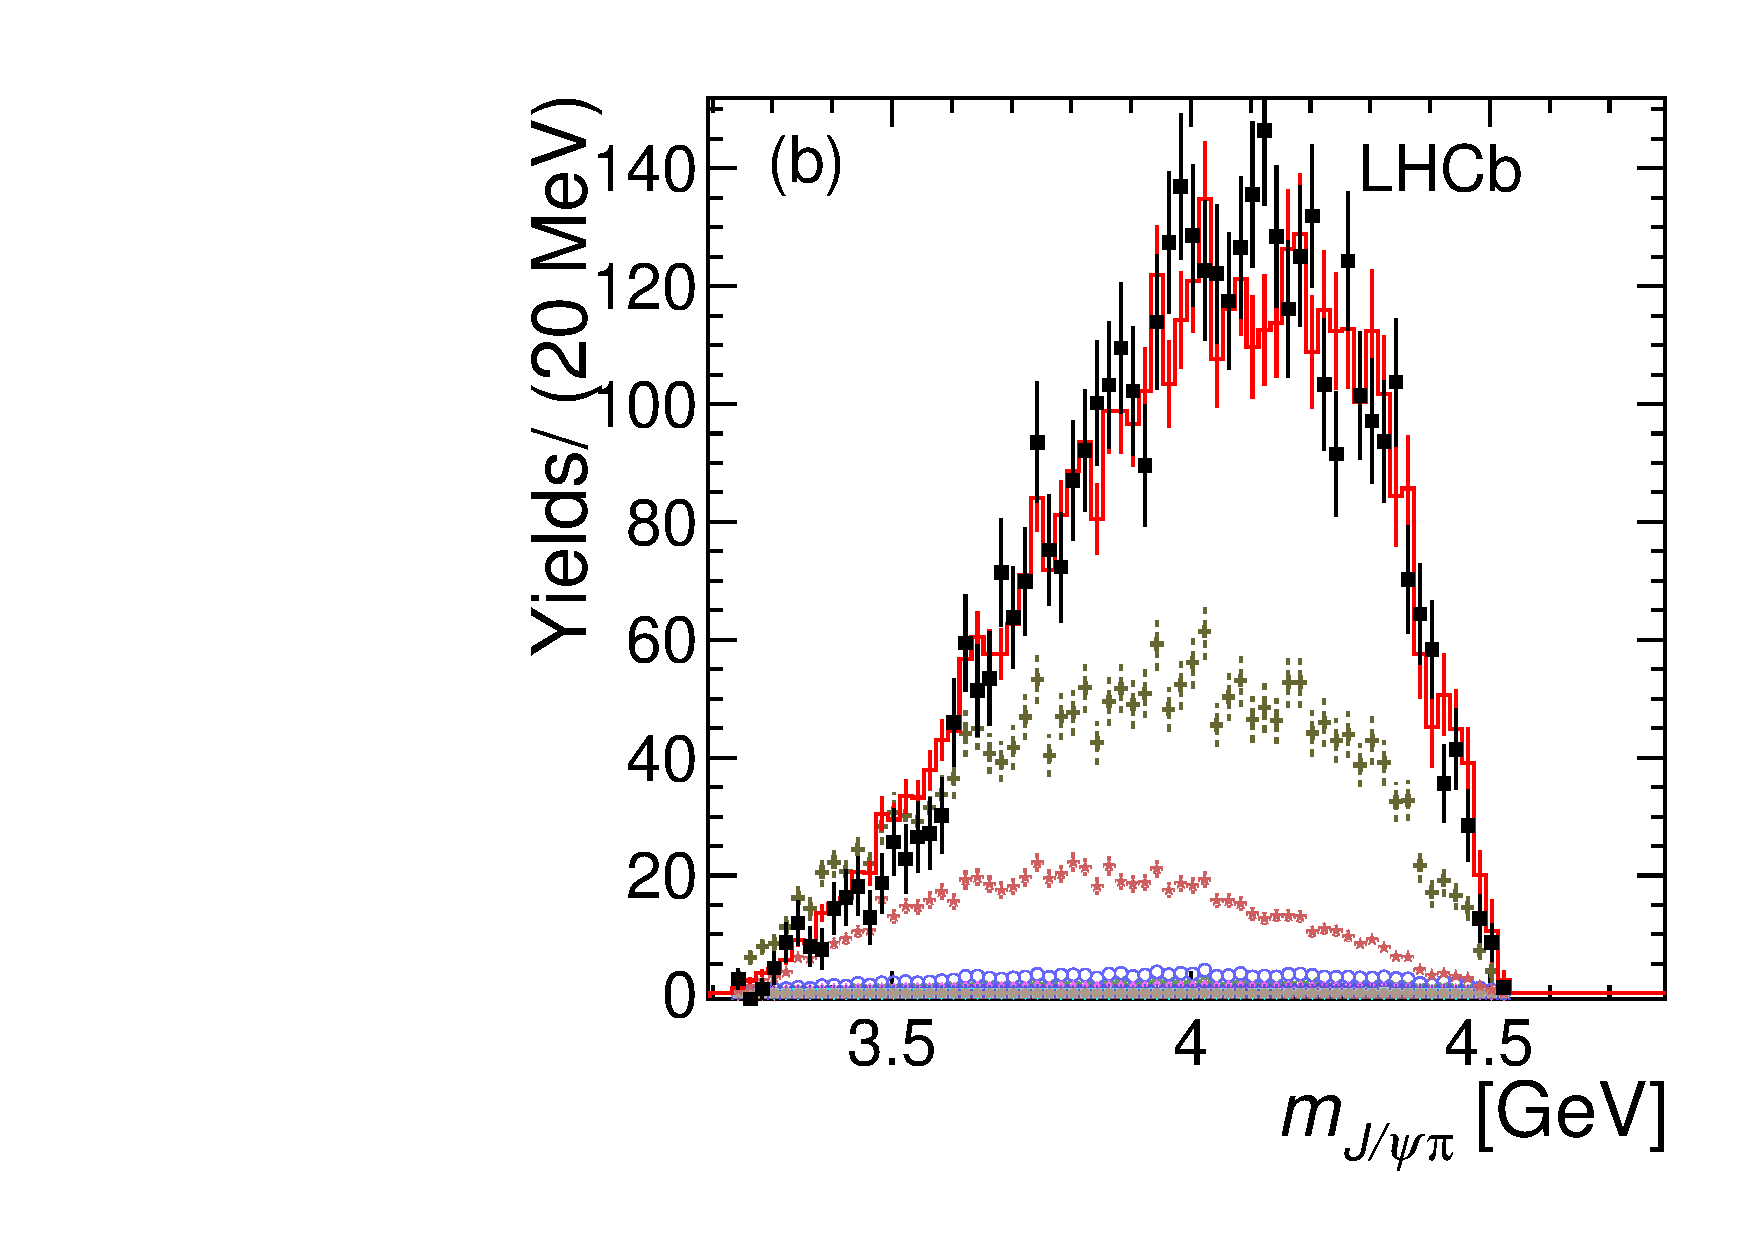
\includegraphics[width=0.4\textwidth]{Figures/04_Penta/05_fit_result/no_pc_plots/mjpsik1}
\put(-150,140) {\textrm{\small \bf Unofficial}}
   \\
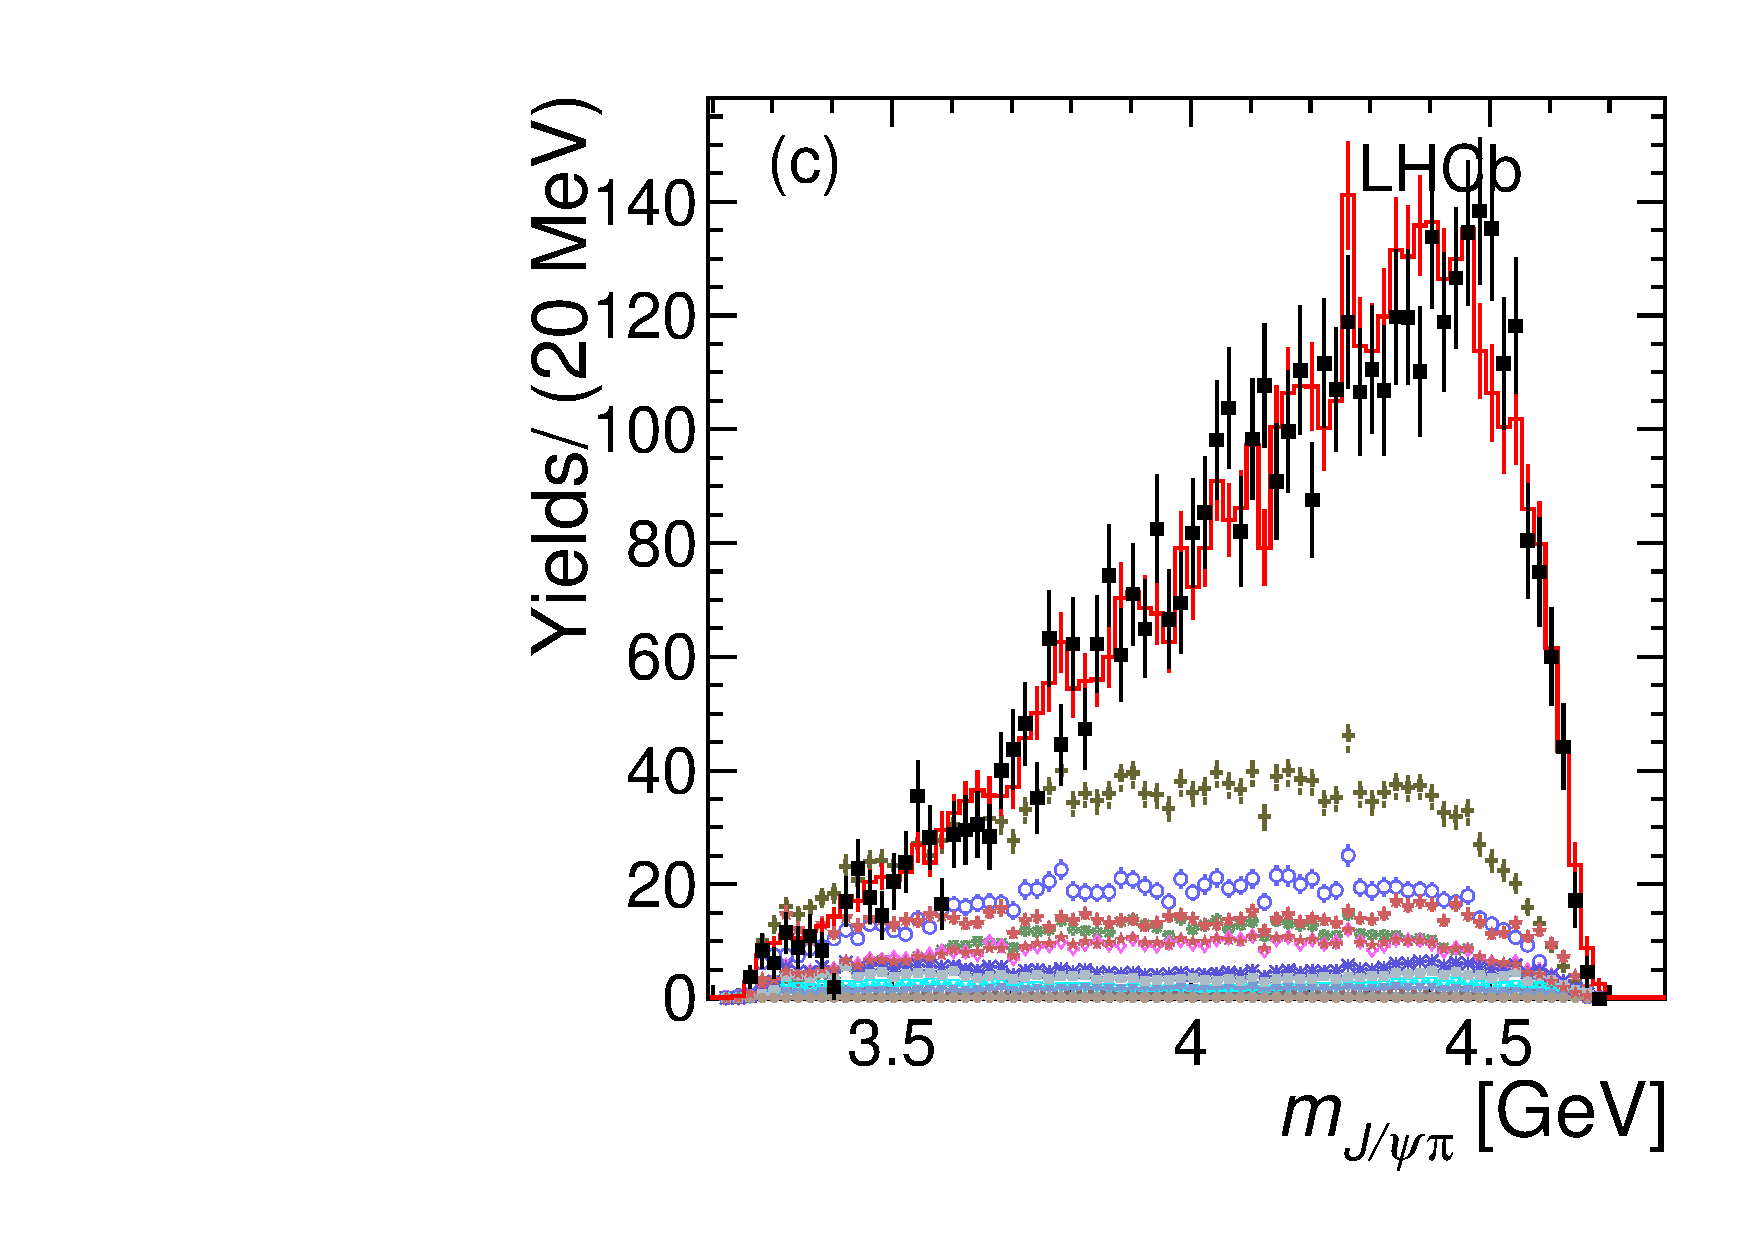
\includegraphics[width=0.4\textwidth]{Figures/04_Penta/05_fit_result/no_pc_plots/mjpsik2}%
\put(-150,140) {\textrm{\small \bf Unofficial}}
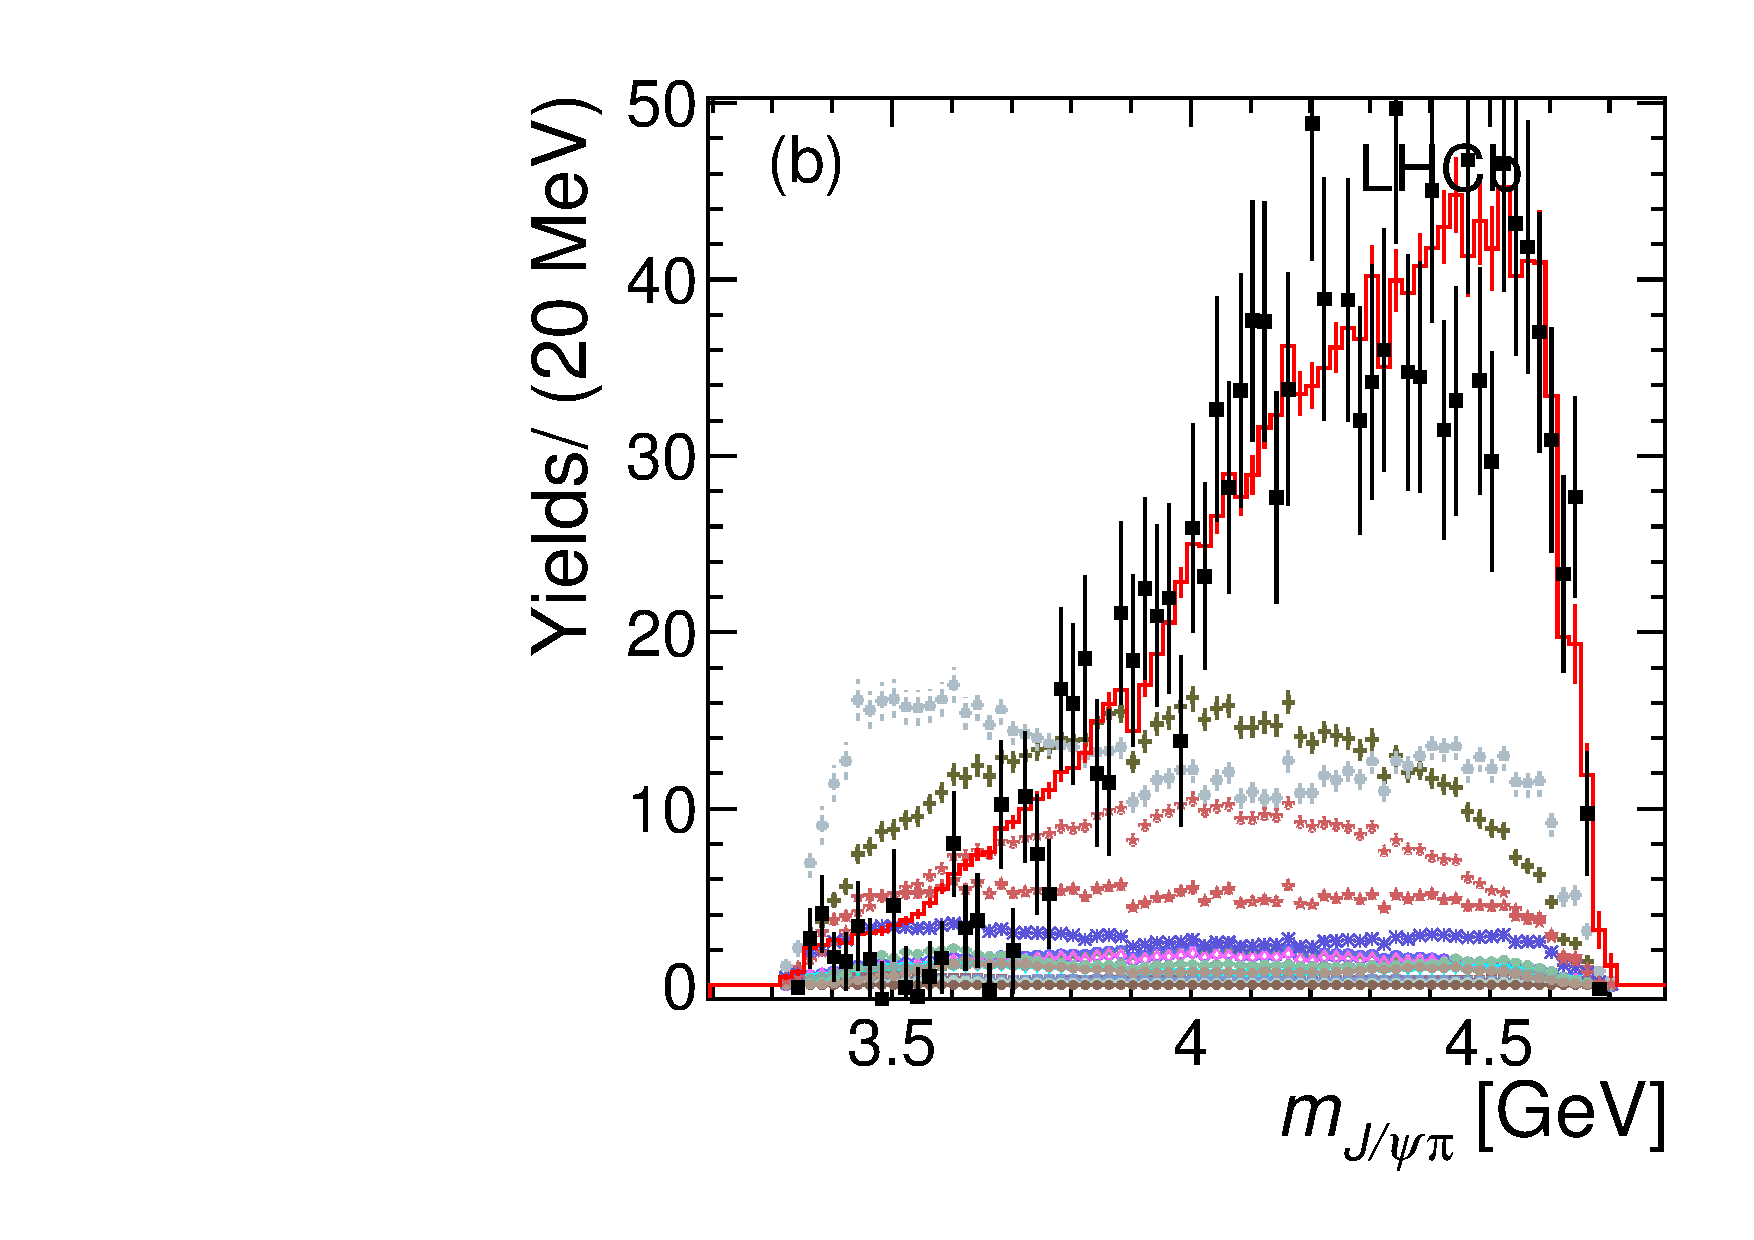
\includegraphics[width=0.4\textwidth]{Figures/04_Penta/05_fit_result/no_pc_plots/mjpsik3}
\put(-150,140) {\textrm{\small \bf Unofficial}}
\end{center}
\vskip -0.5cm
   \caption{$m_{\jpsi \pi}$ in various intervals of $m_{\proton\pi}$ with $N^{*}$ resonances: 
   (a) all $m_{\proton\pi}$ (b) $m_{p\pi}<1.45$\gev, (c) $1.45<m_{p\pi}<1.80$\gev, and (d) $m_{p\pi}>1.80$\gev regions. 
   The data are shown as (black) squares, while the (red) lines show the results of the fit. } 
\label{noZ-mjpsipi-bins}
\end{figure}

As for the $m_{\jpsi\proton}$ projection, 
the $\ZP(4380)$ contribution in the $m_{p\pi}>1.80$\gev region is found to be similar to a contribution 
from a broad $\ZC$  state peaking at approximately $4.2\gev$. 
This is concerning since the Belle collaboration has reported an observation of a charged $1^+$ $\jpsi \pip$ resonant state, 
with the measured mass of $4196_{-29-13}^{+31+17}$\mev and width of $370_{-70-132}^{+70+70}$\mev, 
denoted as $\ZC(4200)^-$~\supercite{Chilikin:2014bkk}.  
Therefore,
it is necessary to investigate if such state can describe the enhancement seen in $m_{\jpsi p}$ for the high $m_{\jpsi\pi}$. 



\subsection{{Fits results considering both four $\ZP$ and $\ZC(4200)$ states}}
%The ``Dalitz" plot of $p\pi^-$ vs $\jpsi \pi^-$ invariant mass-squared is shown in Fig.~\ref{dlz}. 
The $\ZC(4200)$ state is included with various combinations of the $\ZP$ states and the $N^*$ to fit the data, 
where the mass and width of the $\ZC$ state are fixed to that obtained from the Belle collaboration.  
Considerng to determine all the $\ZC$ couplings described by 2 free parameters,
and the maximum orbital angular momentum is set to be 2 
as described in Section.~\ref{sec:Pcpar}, 
the mass and width of the $\ZP$ states are fixed,
%as well as the couplings describing the $\ZP\to\jpsi p$ decay to that obtained from the favored \LbJpsipK modes. 
This leaves 2 free parameters for each $\ZP$ to be determined. 
%In the \LbJpsipK study, 
%the best solution for the $J^P$ of the two $\ZP$ states are $3/2^-$ and $5/2^+$, 
%for the lower and higher mass states, respectively.  
%The parity reversed combination ($3/2^+$, $5/2^-$) only has 1 unit worse for the $\twolnL$ value than the best solution. 
%The other two combinations ($5/2^+$, $3/2^-$) is not ruled out. 
%These three combinations are studied here. 
%We find still these possibilities are not be able to rule out. 
%In addition we add the fourth combination ($5/2^-$, $3/2^+$) as an additional check.  
The NM $N^*+4\ZP+\ZC$ with the molecular model $J^P$ assignment founded in the \LbJpsipK is used as the nominal fit.
The fit projections including NM $N^*+2\ZP+\ZC(4200)$ are shown from Figures.~\ref{fig:fitpczc} to~\ref{PcZc-mjpsipi-bins}. 
The data are well represented by the fit.

\begin{figure}[!tbh]
\centering
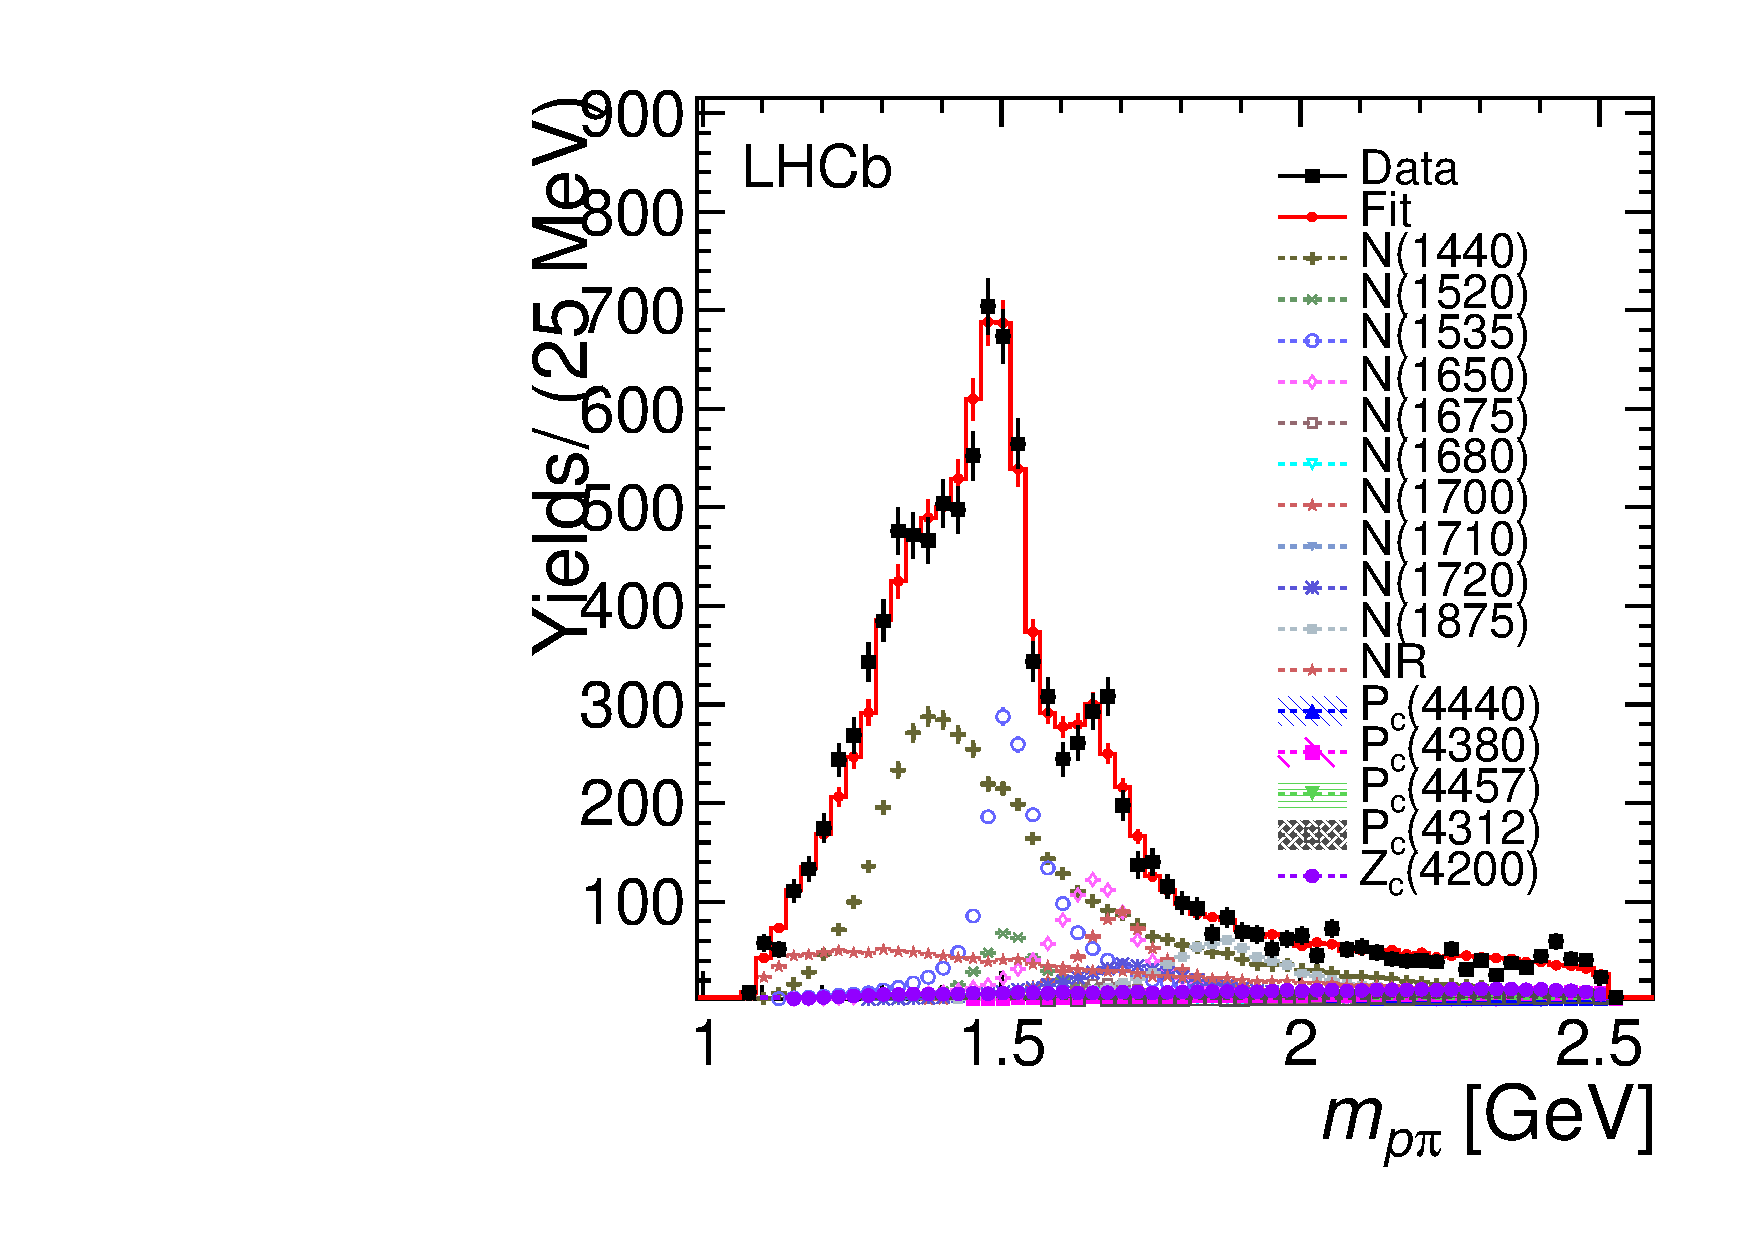
\includegraphics[width=0.4\textwidth]{Figures/04_Penta/05_fit_result/cor_plus2_plots/mppi_S}%
\put(-150,140) {\textrm{\small \bf Unofficial}}
%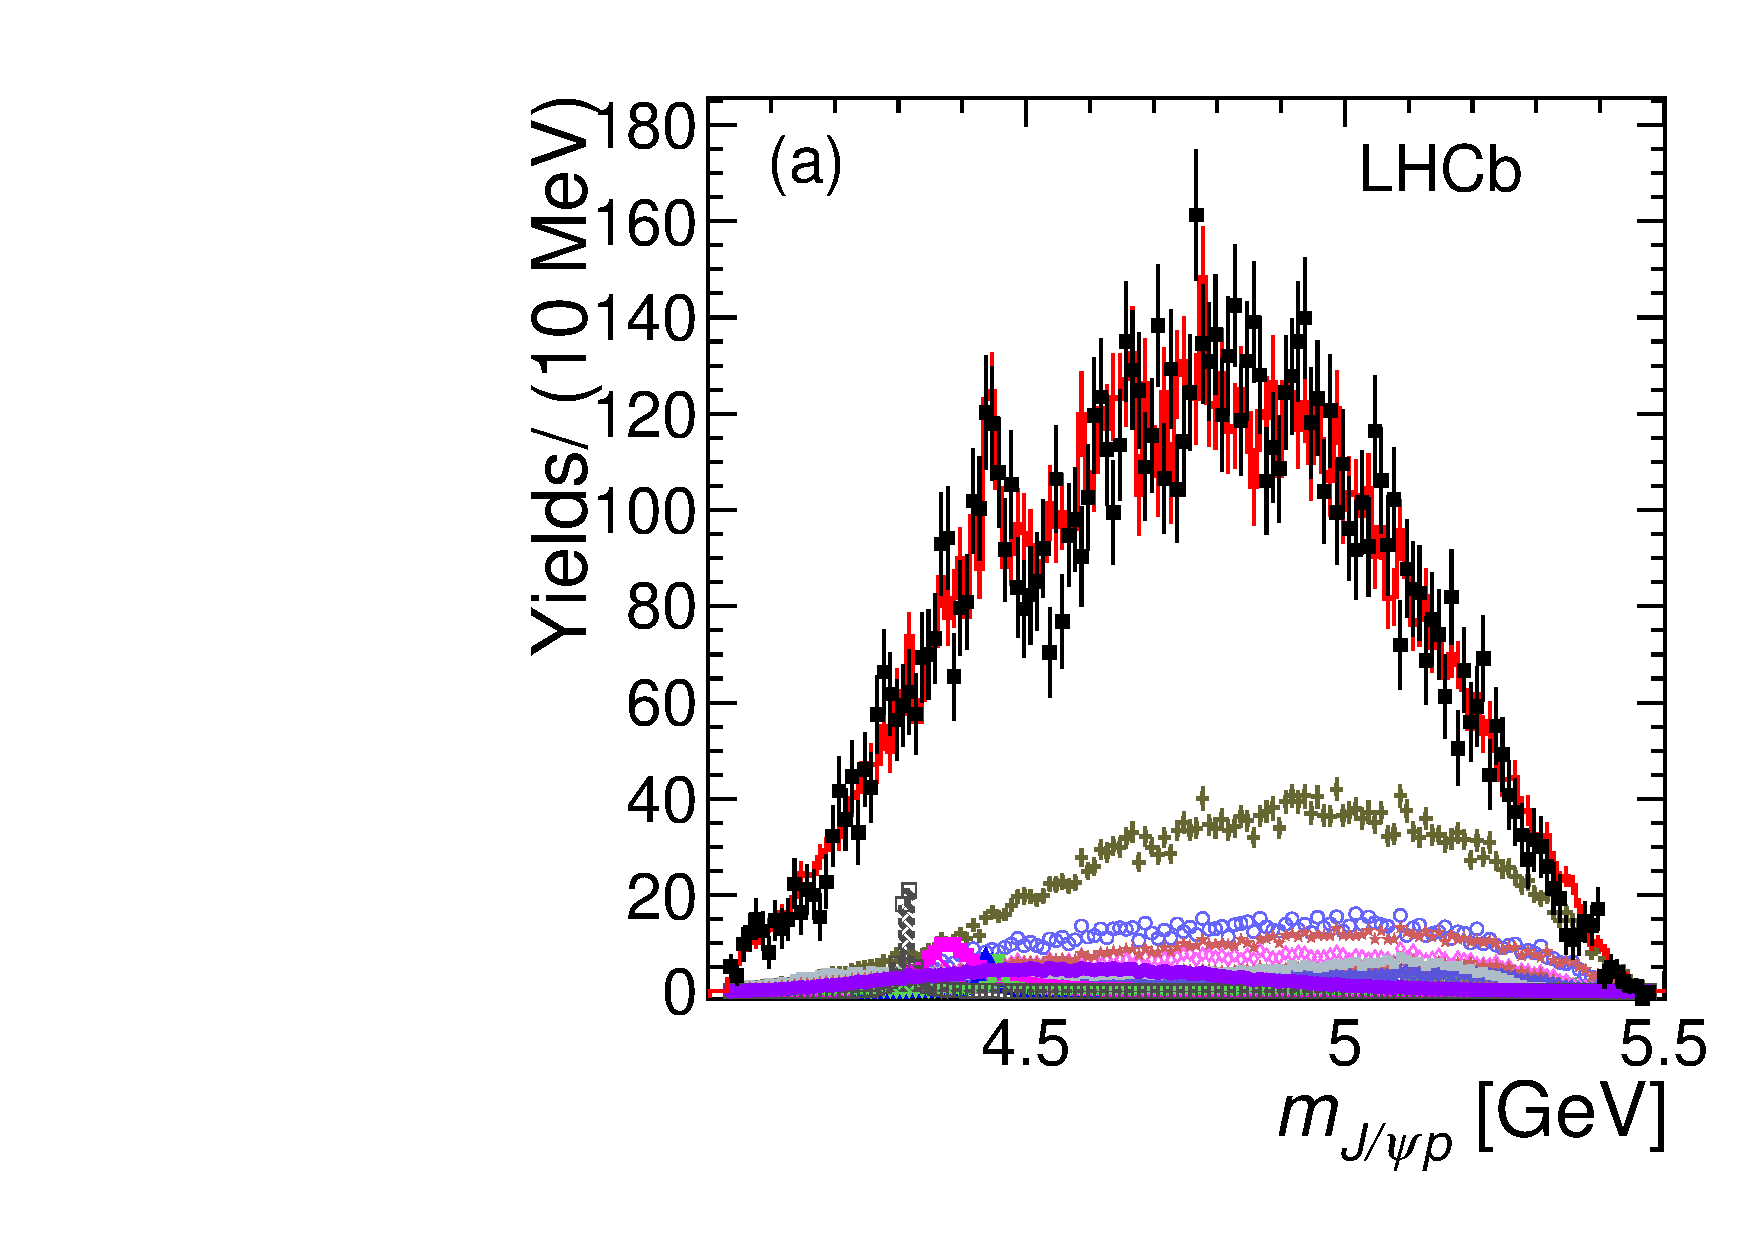
\includegraphics[width=0.48\textwidth]{Figures/04_Penta/05_fit_result/cor_plus2_plots/mjpsip0}%
\vskip -0.5cm
   \caption{Fit projections for $m_{\proton\pi}$ for the default $N^*$ + 2$\ZP$ + $\ZC(4200)$ model. 
   The data are shown as solid (black) squares, 
   while the solid (red) line show the results of the fit. 
   The background is subtracted by sPlot technique. }\label{fig:fitpczc}
\end{figure}

\begin{figure}[!tbh]
\begin{center}
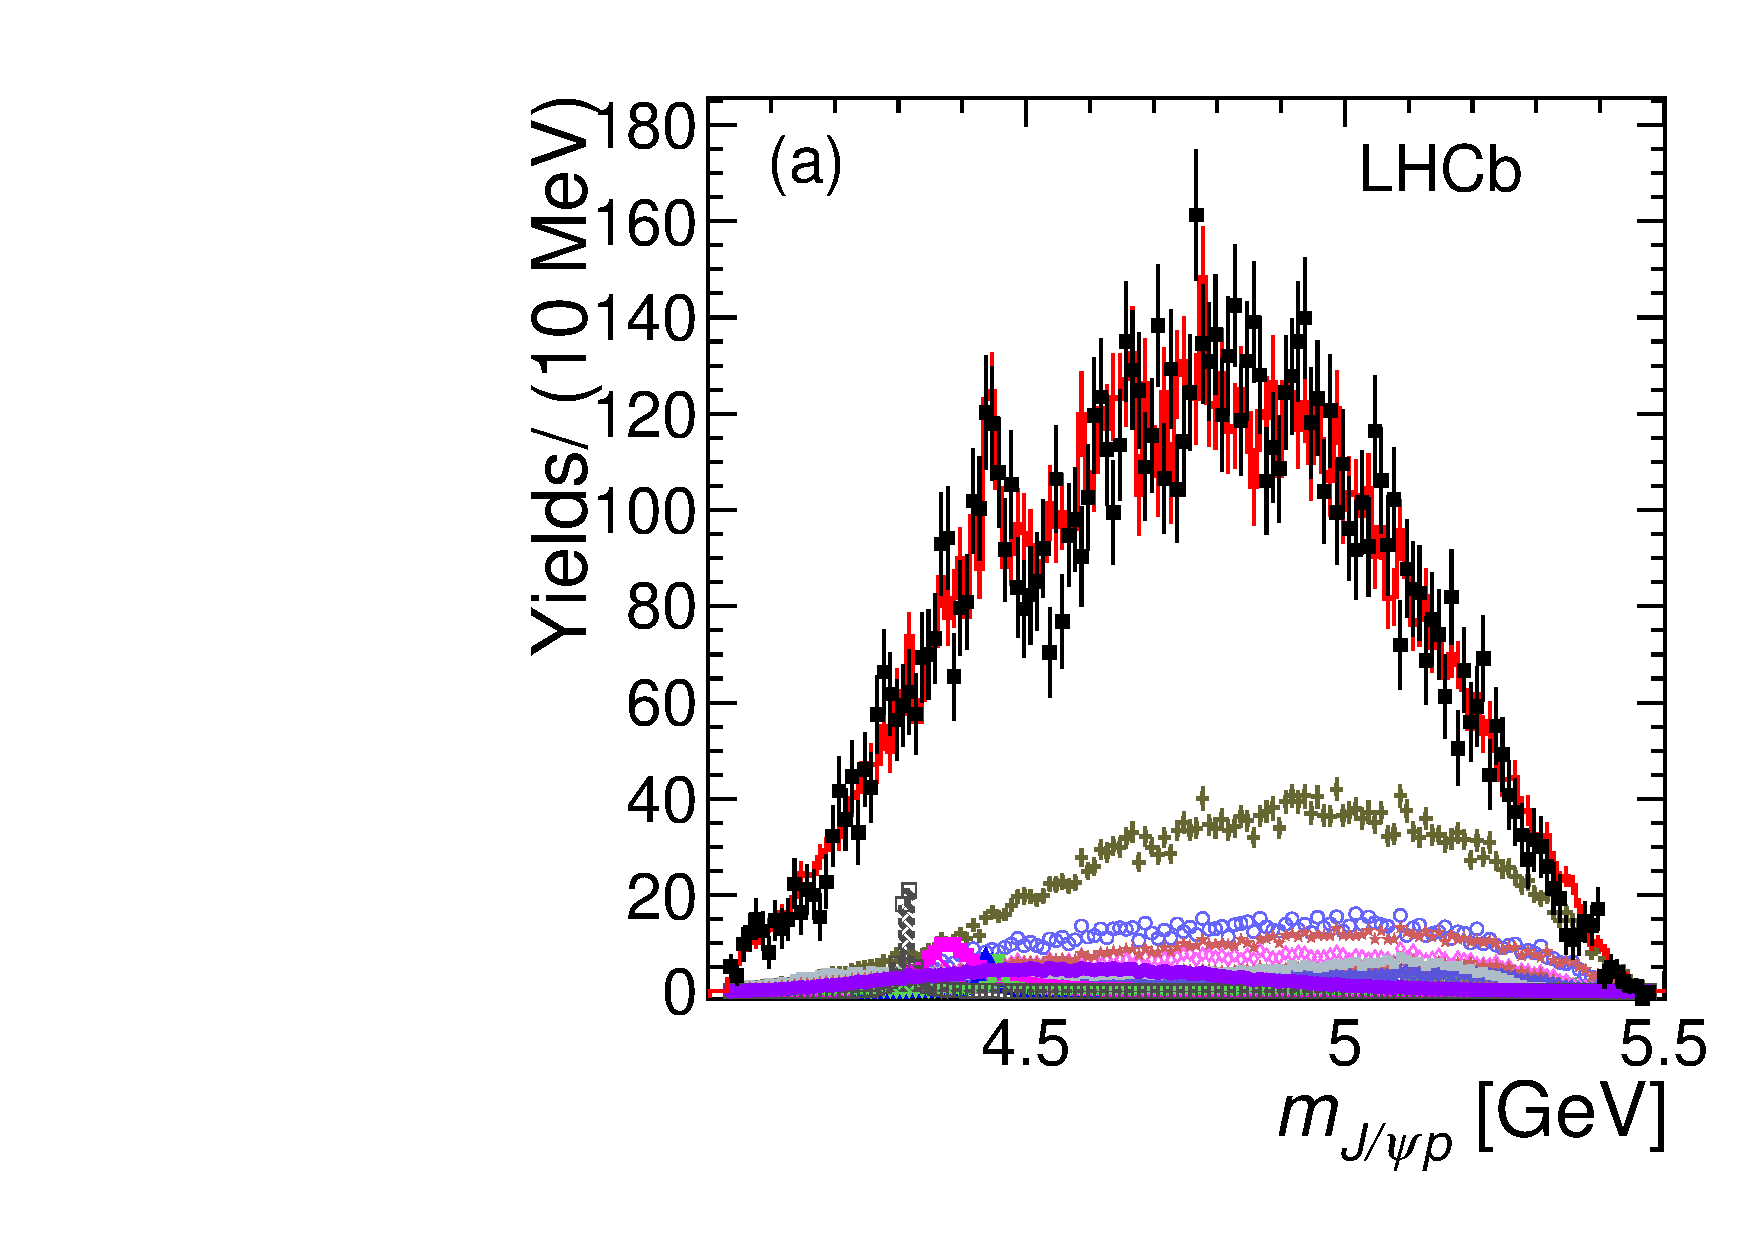
\includegraphics[width=0.4\textwidth]{Figures/04_Penta/05_fit_result/cor_plus2_plots/mjpsip0}%
\put(-60,140) {\textrm{\small \bf Unofficial}}
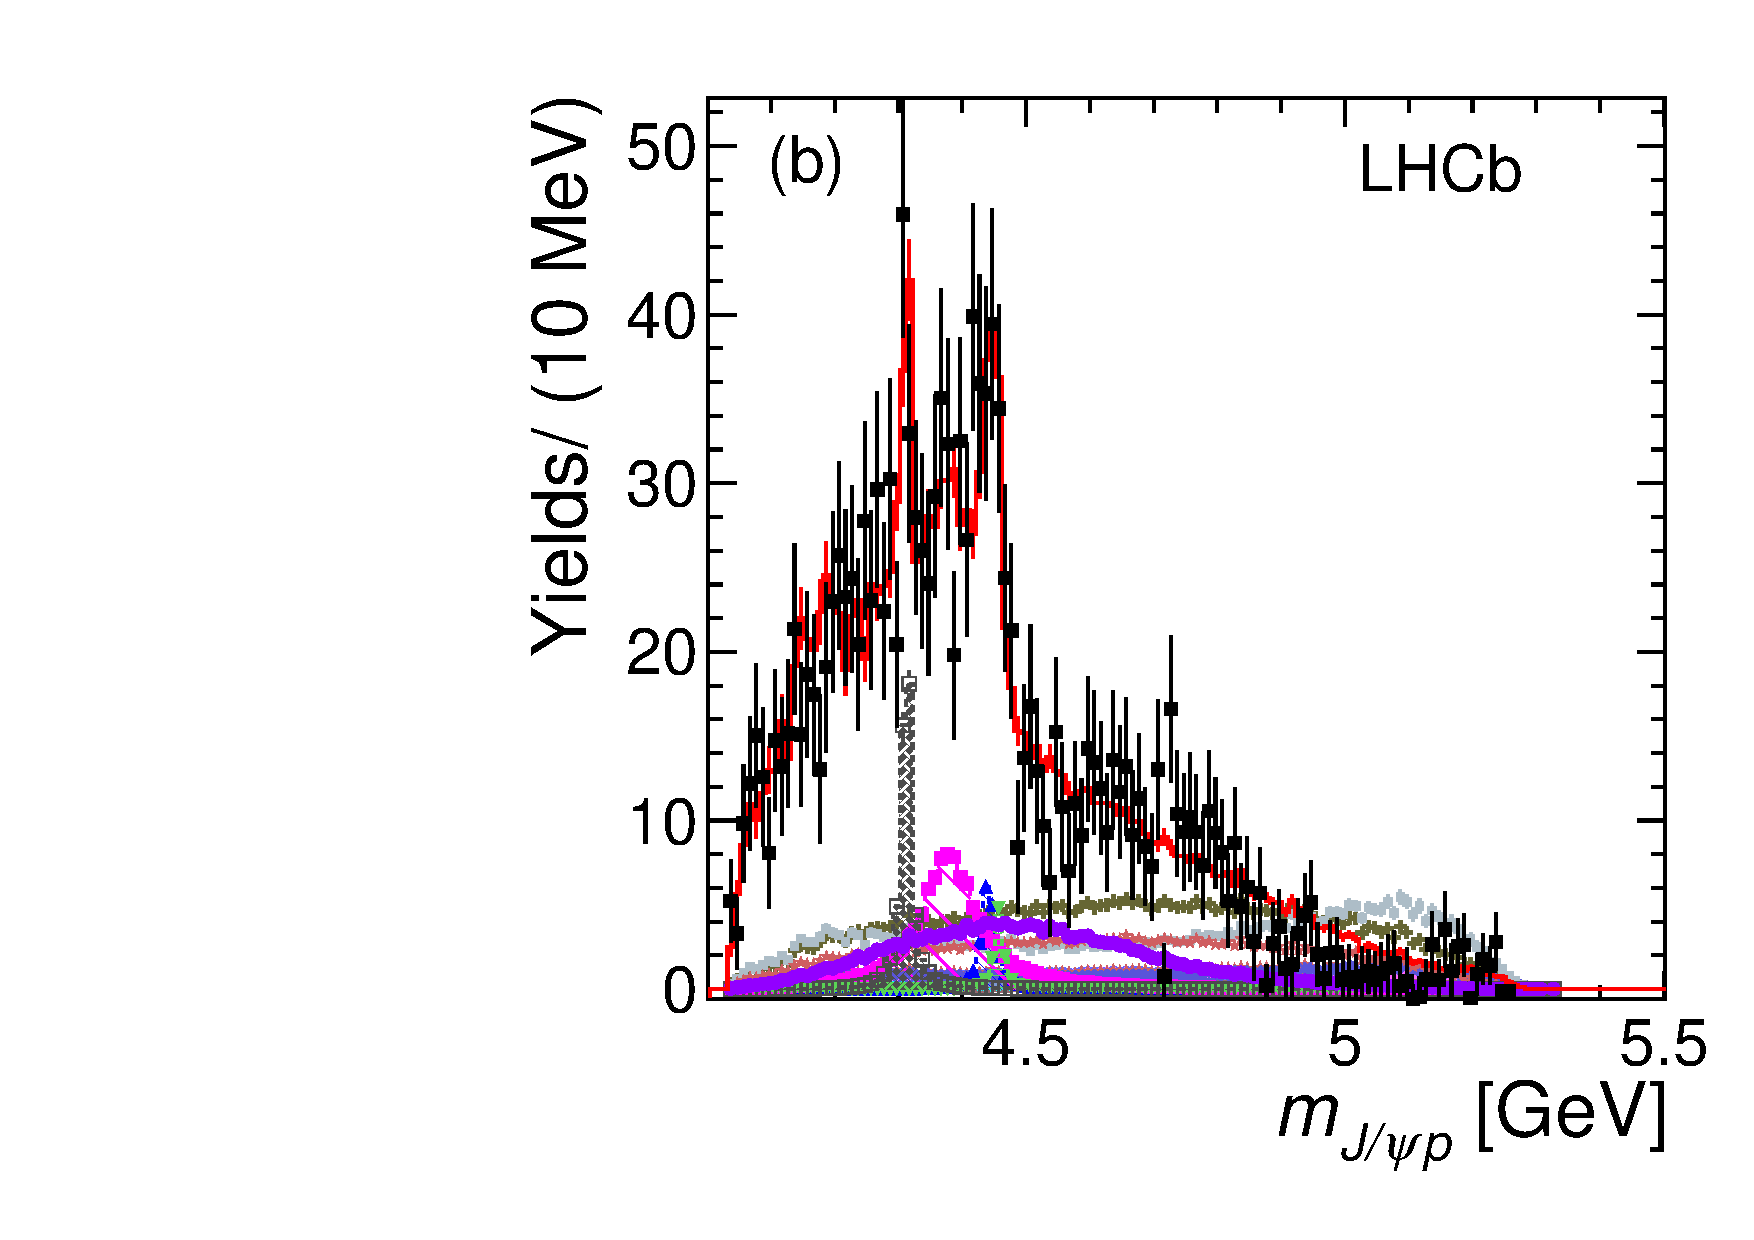
\includegraphics[width=0.4\textwidth]{Figures/04_Penta/05_fit_result/cor_plus2_plots/mjpsip3}
\put(-60,140) {\textrm{\small \bf Unofficial}}
   \\
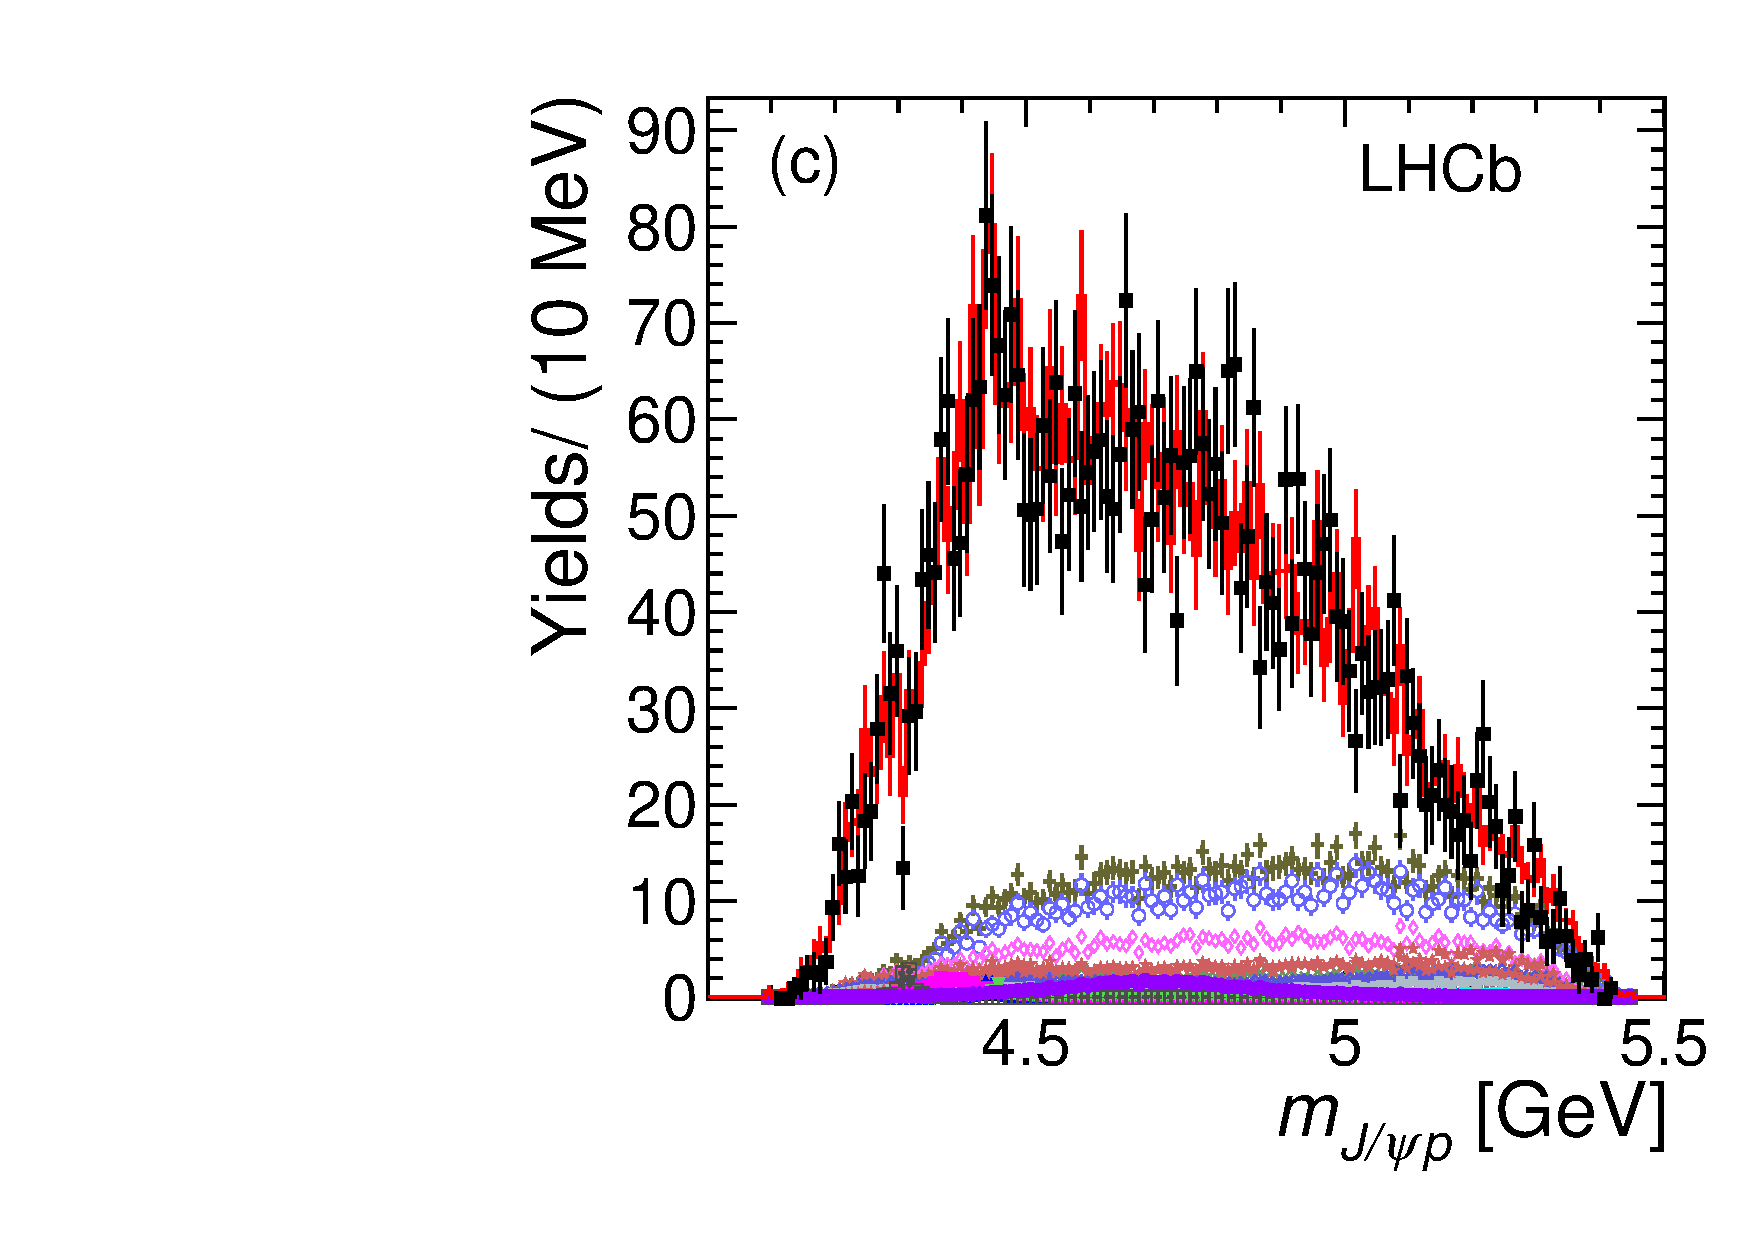
\includegraphics[width=0.4\textwidth]{Figures/04_Penta/05_fit_result/cor_plus2_plots/mjpsip2}
\put(-60,140) {\textrm{\small \bf Unofficial}}
\end{center}
\vskip -0.5cm
   \caption{$m_{\jpsi p}$ in various intervals of $m_{\proton\pi}$ for the  $N^*+2\ZP+\ZC(4200)$ fit: 
   (a) no $m_{p\pi}$\gev cut, (b) $m_{p\pi}>1.80$\gev, and (c) $1.45<m_{p\pi}<1.80$\gev. 
   The data are shown as (black) squares, while the (red) lines show the results of the fit.}
\label{PcZc-mjpsip-bins}
\end{figure}

\begin{figure}[!tbh]
\begin{center}
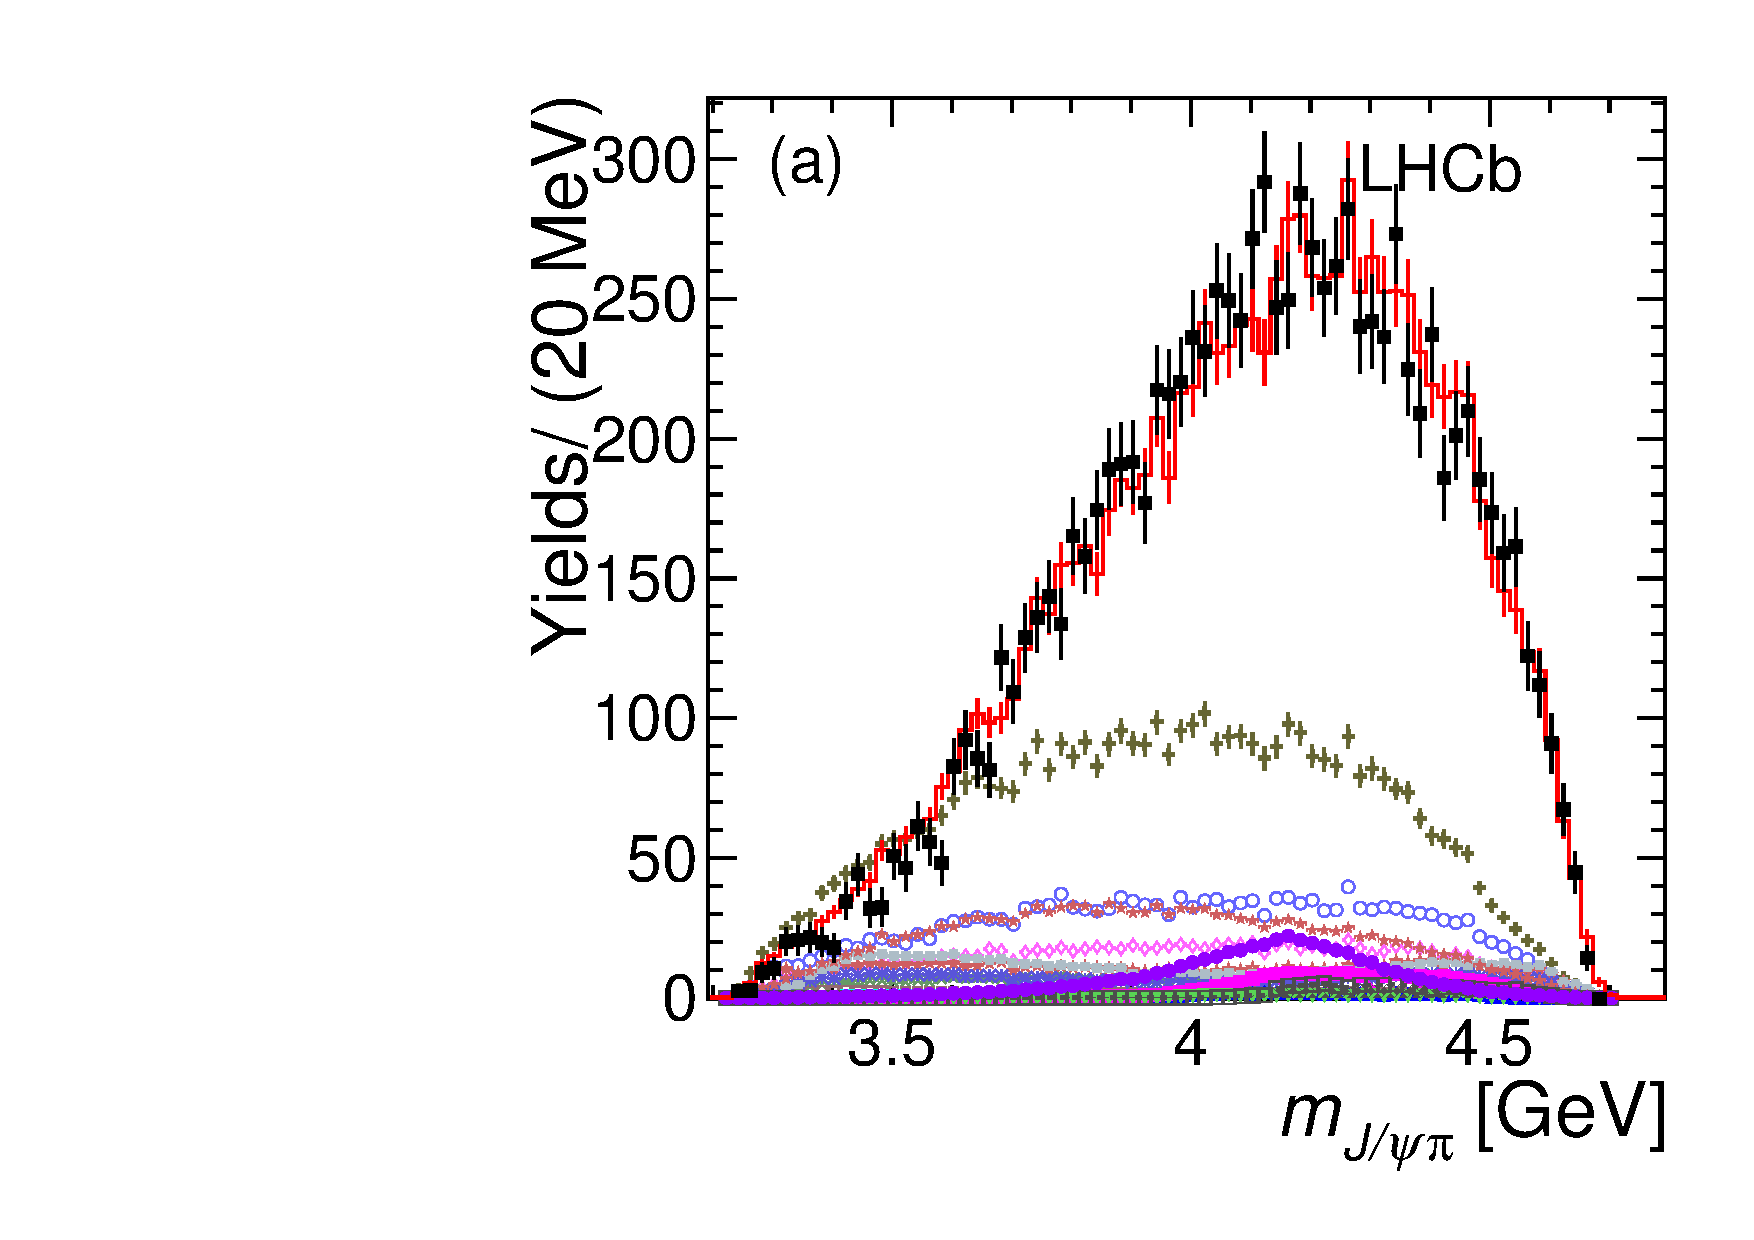
\includegraphics[width=0.4\textwidth]{Figures/04_Penta/05_fit_result/cor_plus2_plots/mjpsik0}%
\put(-150,140) {\textrm{\small \bf Unofficial}}
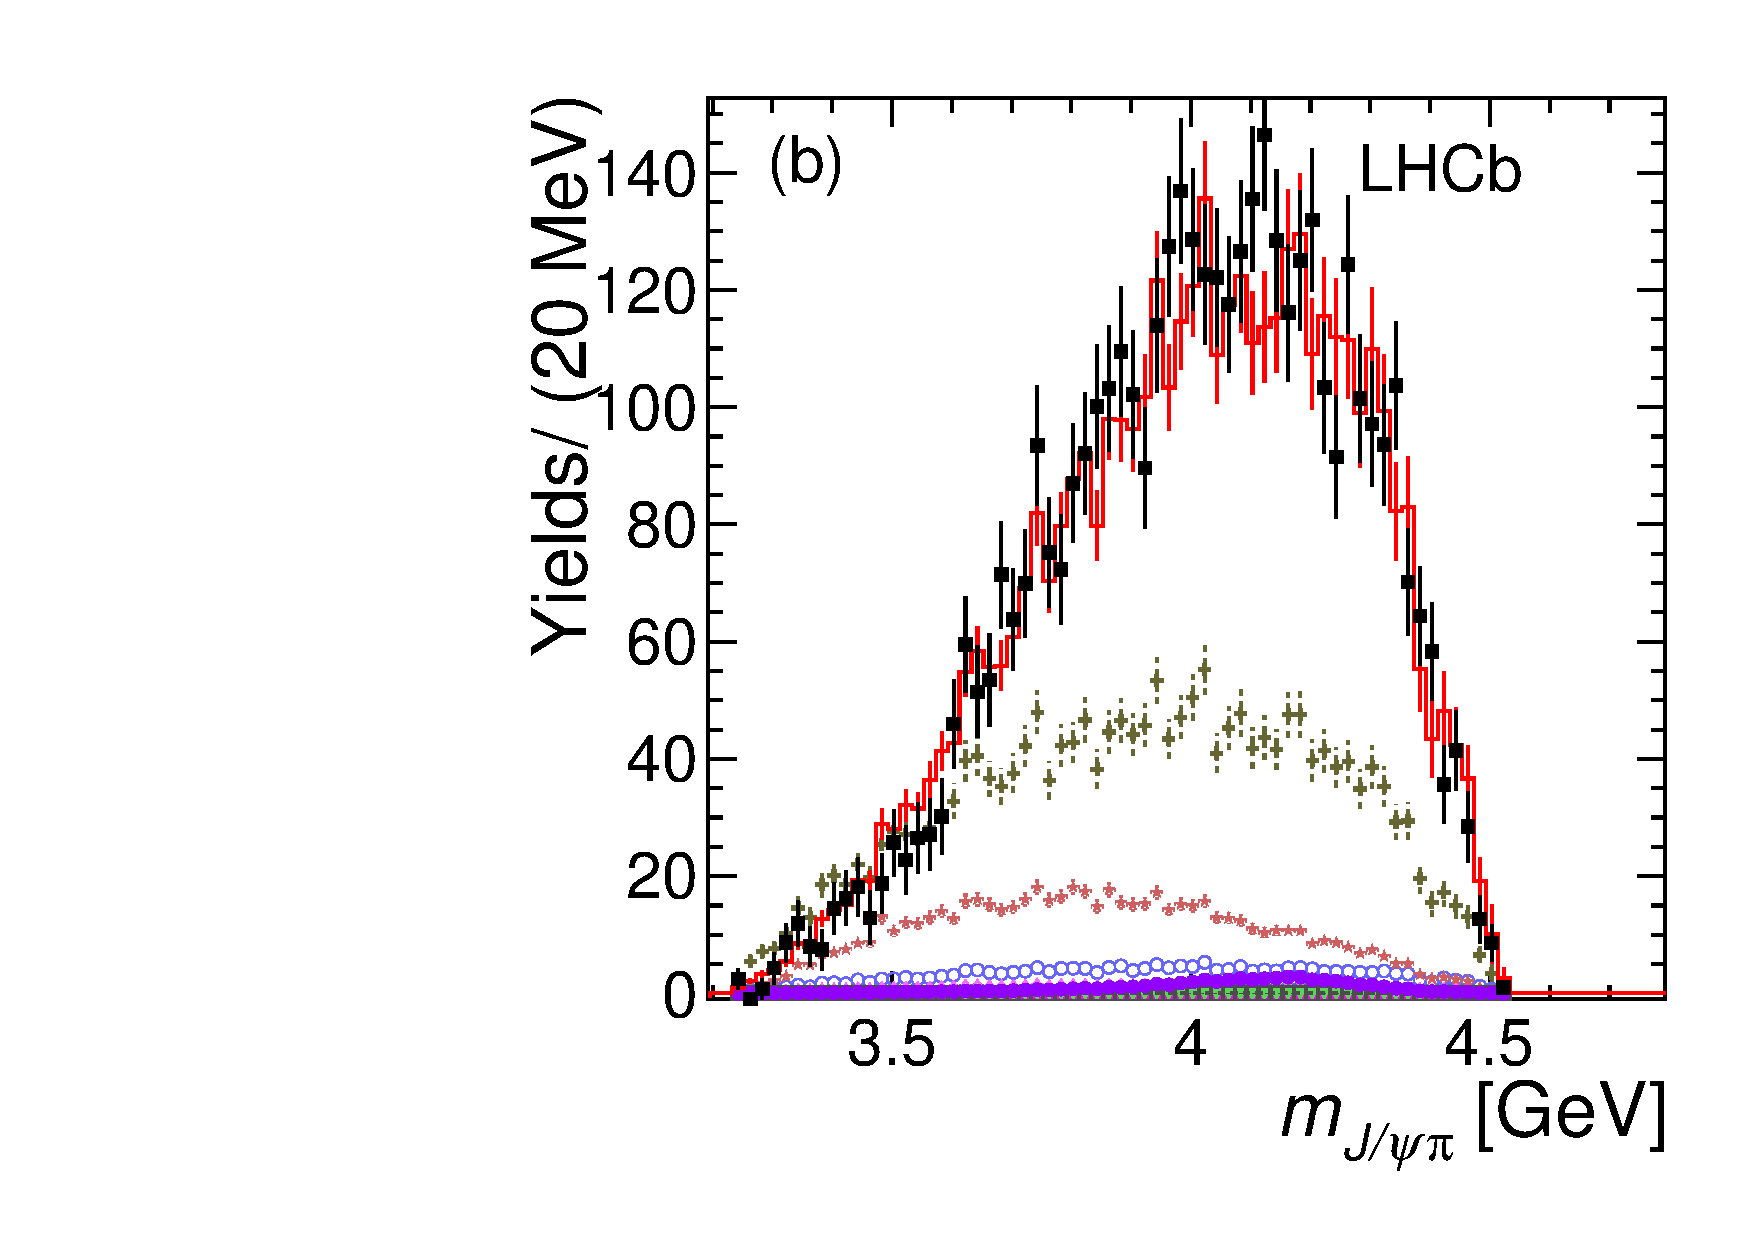
\includegraphics[width=0.4\textwidth]{Figures/04_Penta/05_fit_result/cor_plus2_plots/mjpsik1}
\put(-150,140) {\textrm{\small \bf Unofficial}} \\
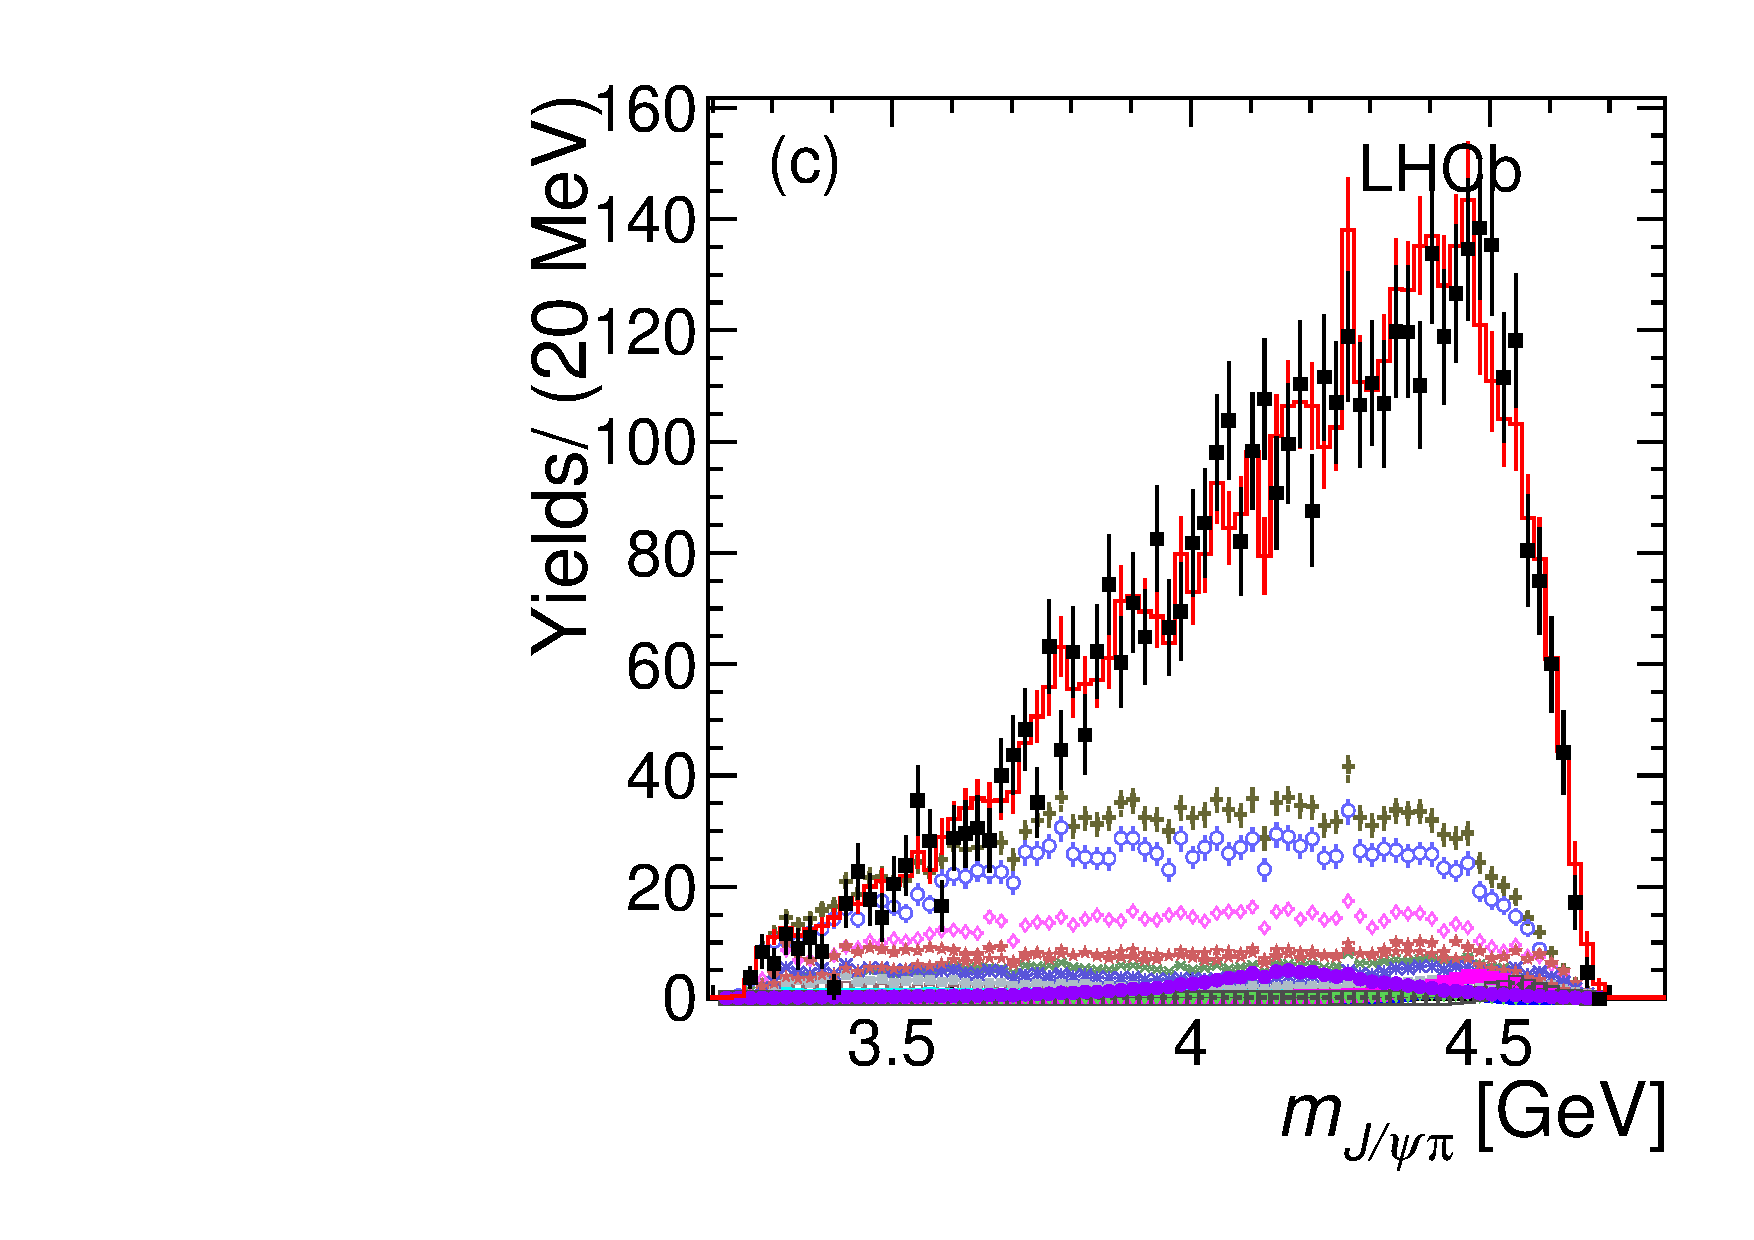
\includegraphics[width=0.4\textwidth]{Figures/04_Penta/05_fit_result/cor_plus2_plots/mjpsik2}%
\put(-150,140) {\textrm{\small \bf Unofficial}}
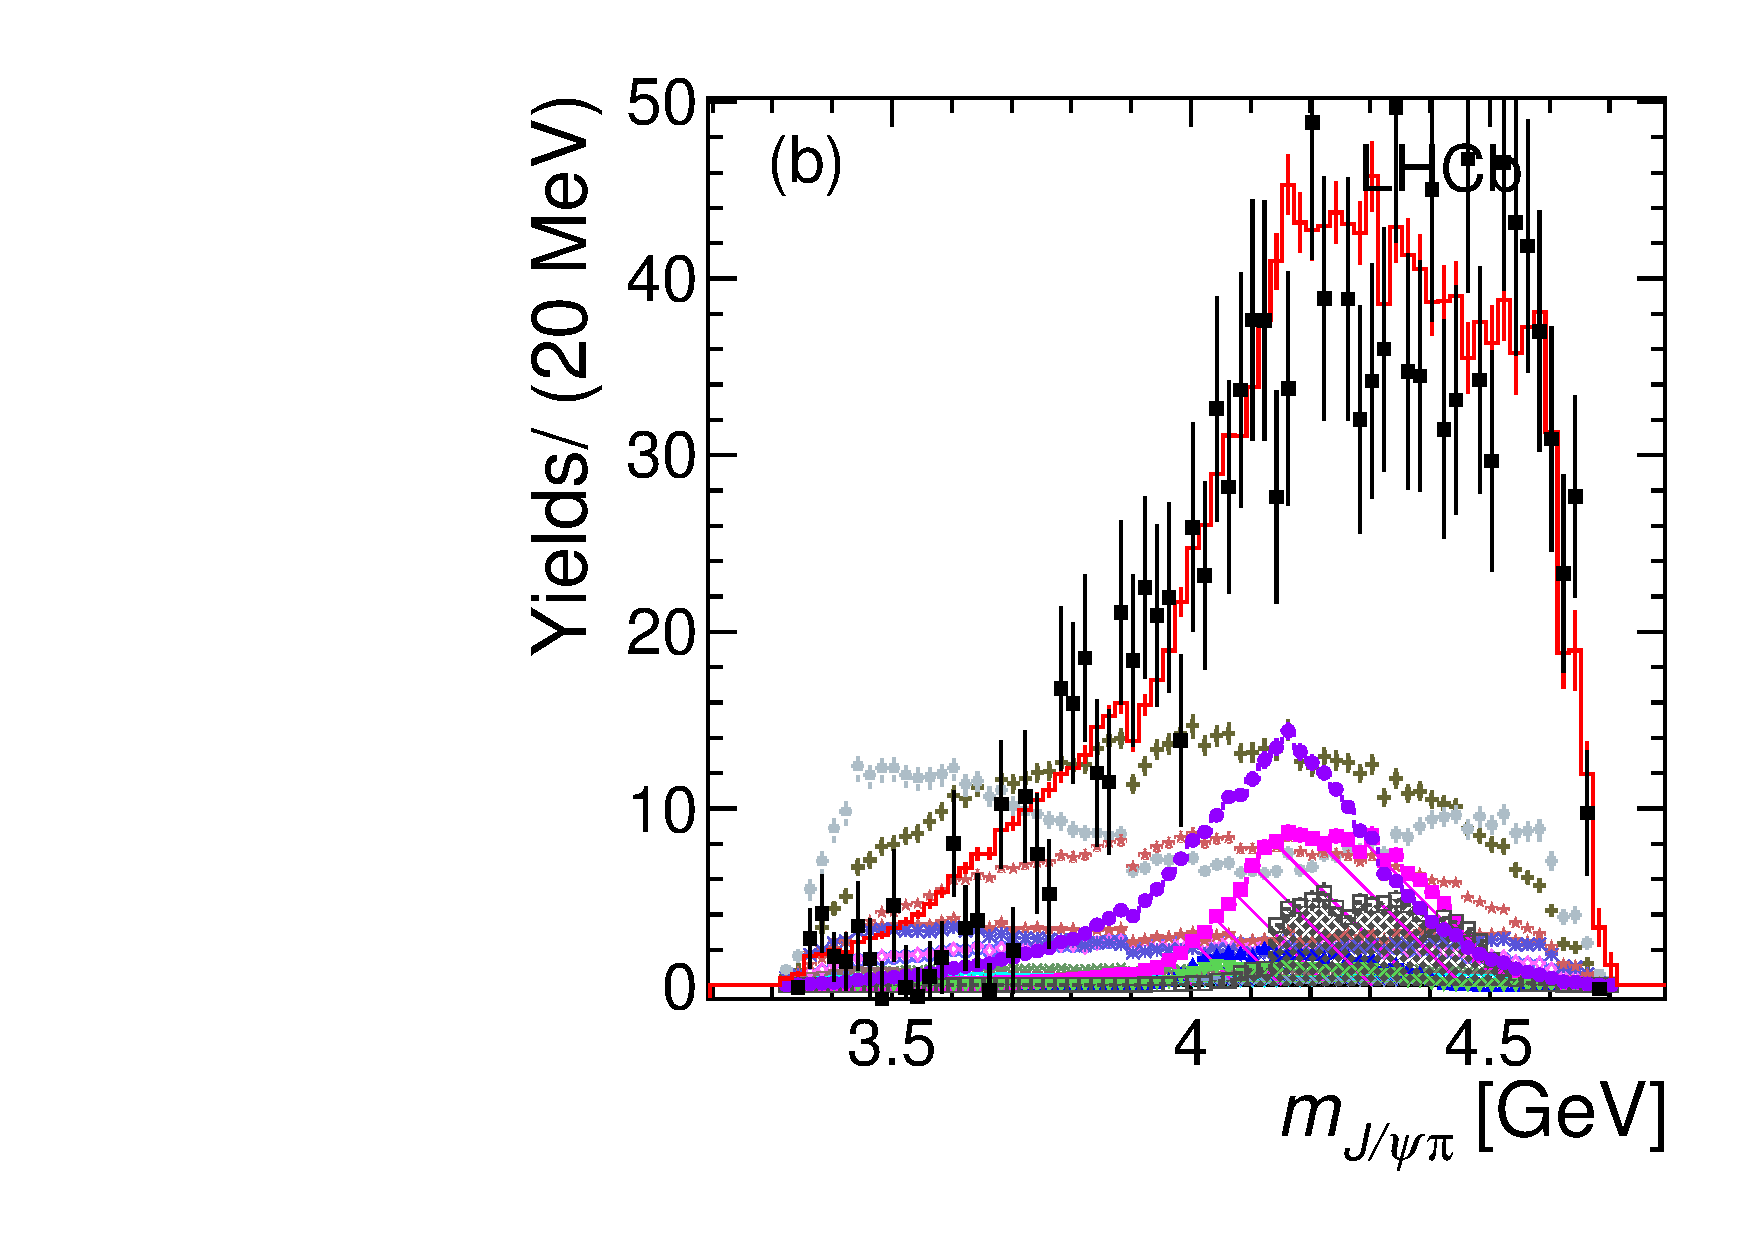
\includegraphics[width=0.4\textwidth]{Figures/04_Penta/05_fit_result/cor_plus2_plots/mjpsik3}
\put(-150,140) {\textrm{\small \bf Unofficial}}
\end{center}
\vskip -0.5cm
\caption{$m_{\jpsi \pi}$ in various intervals of $m_{p\pi}$ for the  $N^*+2\ZP+\ZC(4200)$ fit: 
   (a) all $m_{p\pi}$ (b) $m_{p\pi}<1.45$\gev, (c) $1.45<m_{p\pi}<1.80$\gev, and (d) $m_{p\pi}>1.80$\gev regions. 
   The data are shown as (black) squares, while the (red) lines show the results of the fit.}
   \label{PcZc-mjpsipi-bins}
\end{figure}

 
%\begin{figure}[!tbp]
%\begin{center}
%\includegraphics[width=0.33\textwidth]{NPcZc/ang0}%
%\includegraphics[width=0.33\textwidth]{NPcZc/ang1}%
%\includegraphics[width=0.33\textwidth]{NPcZc/ang2}\\
%\includegraphics[width=0.33\textwidth]{NPcZc/ang3}%
%\includegraphics[width=0.33\textwidth]{NPcZc/ang4}
%\end{center}
%\vskip -0.5cm
%\caption{Various decay angular distributions for the $N^*+2\ZP+\ZC(4200)$ fit. 
%   The data are shown as (black) squares, while the (red) lines show the results of the fit.  
%   See Fig.~\ref{fig:fitpczc} for the legend. The angles are defined in the text.}
%\label{PcZc-angular}
%\end{figure}
%
%
%\begin{figure}[!tbp]
%\begin{center}
%\includegraphics[width=0.33\textwidth]{NPcZc/ang0_3}%
%\includegraphics[width=0.33\textwidth]{NPcZc/ang1_3}%
%\includegraphics[width=0.33\textwidth]{NPcZc/ang2_3}\\
%\includegraphics[width=0.33\textwidth]{NPcZc/ang3_3}%
%\includegraphics[width=0.33\textwidth]{NPcZc/ang4_3}
%\end{center}
%\vskip -0.5cm
%\caption{Various decay angular distributions for the $N^*+2\ZP+\ZC(4200)$ fit in $\mppi>1.8$\gev. 
%   The data are shown as (black) squares, while the (red) lines show the results of the fit.  
%   See Fig.~\ref{fig:fitpczc} for the legend. The angles are defined in the text.}
%\label{PcZc-angular-3}
%\end{figure}

In order to calculate $p$-value for the log likelihood-ratio obtained on the data, 
probability density of $\Delta(\twolnL)$ must be known under H0 (e.g. no-exotic) hypothesis. 
It is a common practice to use Wilks’ theorem, 
which states that for continuous hypotheses i.e. 
when H0 is a special case of more general H1 (H0 is “nested” in H1) asymptotically 
for infinite statistics ($N\to\infty$) $\Delta(\twolnL)$ has a $\chi^2$ distribution 
with a number of degrees of freedom (ndf) equal to the number of constrained parameters in H0 hypotheses relatively to the H1. 
This leads to the following formula for significance expressed in standard deviations:
\begin{equation}
n_{\sigma}(\Delta(\twolnL)) =
\sqrt{2} \texttt{ROOT::TMath::ErfcInverse(ROOT::TMath::Prob}(\Delta(\twolnL), {\rm ndf})) . 
\end{equation}
This is verified by a large sets of toy MC. 

The results of the $\Delta(\twolnL)$, 
between the fits including various combinations of the exotic states and the fit including only the $N^*$ resonances, 
are shown in Tables~\ref{tab:LL_nor} and~\ref{tab:sig_nor} for the NM. 
%respectively\footnote{The $N^*+2\ZP+\ZC$ fit for ($3/2^-$, $5/2^+$) couldn't converge for EM, 
%while it can provide the lowest bound for $\Delta(\twolnL)$.}. 
%As for the $\twolnL$, both the $\ZC(4200)$ and the two $\ZP$ states can improve the $N^*$ fit by a large amount; 
%the $\ZP(4380)$ and the $\ZC(4200)$ have almost equal improvements although the $\ZC(4200)$ has 6 more free parameters.  
%In the fits including both types of exotic states,  
%total improvement of the $\twolnL$ is $100.3$ for ndf=18. 
%But because of strong correlation between the two broad states $\ZP(4380)$ and $\ZC(4200)$, 
%individual significance for the two types of exotic states is largely reduced to be statistically insignificant. 
%Thus we consider three hypotheses: 
%assuming either the $\ZC$ state or the $\ZP$ states aren't present in the data, 
%or both could exist. 
%Under each hypothesis, 
%we use the smallest $\Delta(\twolnL)$ among the four $J^P$ combinations, 
%as listed in Tables~\ref{tab:zcfit} and~\ref{tab:zcfit-em}, 
%to calculate the significances of various exotic states for conservative. 
%The results are presented in Table~\ref{tab:zcsig}. 
%The significance values are moderately reduced from NM to EM, 
%where the latter is taken as the final numbers to take into account the systematic uncertainty. 
%For the $2\ZP$ states, 
%the number is 7.2$\sigma$ with the $N^*+2\ZP$ hypothesis, 
%and is reduced to 3.1$\sigma$ with the $N^*+2\ZP+\ZC$, 
%showing an evidence for the $2\ZP$ contribution. 
%While for the $\ZC(4200)$ state, 
%6.4$\sigma$ in the $N^*+\ZC$ hypothesis is reduced to about 1$\sigma$ when including both types of the exotics. 



\begin{table}[htb]
\centering
\caption{ Nominal model : $\Delta$(-2$\log(L)$). }
\label{tab:LL_nor}
\vspace{0.2cm}
\begin{tabular}{lc }
\hline\\[-2.5ex]
 State                                  &   $\Delta$(-2$\log(L)$)  \\
 \hline \\[-2.5ex]
 $N^*$                                  &   0(-13452.92)    \\
 $N^*+4P_c$                             &   -256.09    \\
 $N^*+4P_c-P_c(4440)$                   &   -246.46    \\
 $N^*+4P_c-P_c(4380)$                   &   -174.86    \\
 $N^*+4P_c-P_c(4457)$                   &   -252.38    \\
 $N^*+4P_c-P_c(4312)$                   &   -203.03    \\
 $N^*+4P_c-P_c(4440)-P_c(4457)$         &   -212.66    \\
 \hline
 $N^*+Z_c$                              &   -176.42    \\
 $N^*+Z_c+4P_c$                         &   -294.52    \\
 $N^*+Z_c+4P_c-P_c(4440)$               &   -282.76    \\
 $N^*+Z_c+4P_c-P_c(4380)$               &   -264.07    \\
 $N^*+Z_c+4P_c-P_c(4457)$               &   -282.31    \\
 $N^*+Z_c+4P_c-P_c(4312)$               &   -245.78    \\
 $N^*+Z_c+4P_c-P_c(4440)-P_c(4457)$     &   -250.48    \\
\hline
 $N^*+3P_c-P_c(4440)$                   &   -118.84    \\
 $N^*+3P_c-P_c(4457)$                   &   -156.03    \\
 $N^*+3P_c-P_c(4312)$                   &   -93.73     \\
 $N^*+3P_c-P_c(4440)-P_c(4457)$         &   -61.39     \\
\hline
 $N^*+Z_c+3P_c-P_c(4440)$               &   -231.05    \\
 $N^*+Z_c+3P_c-P_c(4457)$               &   -251.10    \\
 $N^*+Z_c+3P_c-P_c(4312)$               &   -221.16    \\
 $N^*+Z_c+3P_c-P_c(4440)-P_c(4457)$     &   -207.01    \\
 \hline
\end{tabular}
\end{table}


 \begin{table}[htb]
\centering
\caption{ Significance under various hypotheses with nominal model. }
\label{tab:sig_nor}
\vspace{0.2cm}
\begin{tabular}{ l|c|c|c|c }
\hline\\[-2.5ex]
 State                   & $N^*+4P_c$   & $N^*+4P_c+Z_c$  & $N^*+3P_c$   & $N^*+3P_c+Z_c$  \\
 \hline \\[-2.5ex]
 $P_c(4440)$             & 2.7$\sigma$  & 2.2$\sigma$  & 7.2$\sigma$  & 5.4$\sigma$     \\
 $P_c(4380)$             & 8.7$\sigma$  & 5.1$\sigma$  & -            & -               \\
 $P_c(4457)$             & 1.3$\sigma$  & 3.1$\sigma$  & 3.9$\sigma$  & 3.2$\sigma$     \\
 $P_c(4312)$             & 7.0$\sigma$  & 6.7$\sigma$  & 8.7$\sigma$  & 6.2$\sigma$     \\
 $P_c(4440)+P_c(4457)$   & 5.6$\sigma$  & 5.8$\sigma$  & 9.9$\sigma$  & 6.8$\sigma$     \\
 $4P_c$                  & 14.9$\sigma$ & 9.8$\sigma$  & -            & -               \\
 $4P_c+Z_c$              & -            & 15.9$\sigma$ & -            & -     \\
 $Z_c$                   & -            & 6.6$\sigma$  & -            & 9.2$\sigma$     \\
\hline
\end{tabular}
\end{table}



%\begin{table}[!tbp]
%\centering
%\caption{$\Delta(\twolnL)$ under various compositions in the fits with respect to the $N^*$ fit for the two $N^*$ models.} 
%\label{tab:zcfit}
%\begin{tabular}{clrr}\hline
%Fit \# & Composition in fit & \RM &\IM \\\hline
%1)	&	$N^*+\ZC$	&	97.9 	&	79.2 	\\	
%2)	&	$N^*+\ZP(4380)$	&	99.6 	&	80.3 	\\	
%3)	&	$N^*+\ZP(4450)$	&	43.3 	&	35.8 	\\	
%4)	&	$N^*+2\ZP$	&	110.2 	&	89.7 	\\	
%5)	&	$N^*+\ZC+\ZP(4380)$	&	115.9 	&	91.2 	\\	
%6)	&	$N^*+\ZC+\ZP(4450)$	&	107.9 	&	92.1 	\\	
%7)	&	$N^*+2\ZP+\ZC$	&	127.0 	&	100.2 	\\	\hline
%\end{tabular}
%\end{table}

%\begin{table}[!tbp]
%\centering
%\caption{$\Delta(\twolnL)$ in the fits with respect to the $N^*$ fit with the \RM under different $J^P$ assignments for ($\ZP(4380)$, $\ZP(4450)$), where the first two assignment are the best two preferences from the previous study.} 
%\label{tab:zcfit}
%\begin{tabular}{clcccc}\hline
%Fit \# & Composition in fit & ($3/2^-$, $5/2^+$) & ($3/2^+$, $5/2^-$) & ($5/2^-$, $3/2^+$) & ($5/2^+$, $3/2^-$)  \\\hline
%1)	&	$N^*+\ZC$	&	~~96.5 	&	~~96.5 	&	~~96.5 	&	~~96.5 		\\	
%2)	&	$N^*+\ZP(4380)$	&	101.4 	&	105.4 	&	~~96.1 	&	~~99.6 		\\	
%3)	&	$N^*+\ZP(4450)$	&	~~44.7 	&	~~42.6 	&	~~46.8 	&	~~45.6 		\\	
%4)	&	$N^*+2\ZP$	&	111.9 	&	117.0 	&	110.8 	&	108.4 		\\	
%5)	&	$N^*+\ZC+\ZP(4380)$	&	117.8 	&	122.5 	&	110.7 	&	117.6 		\\	
%6)	&	$N^*+\ZC+\ZP(4450)$	&	108.3 	&	108.7 	&	102.0 	&	107.7 		\\	
%7)	&	$N^*+2\ZP+\ZC$	&	127.9 	&	133.9 	&	123.7 	&	126.8 		\\	\hline
%\end{tabular}
%\end{table}
%
%\begin{table}[!tbp]
%\centering
%\caption{$\Delta(\twolnL)$ in the fits with respect to the $N^*$ fit with the \EM under different $J^P$ assignments for ($\ZP(4380)$, $\ZP(4450)$), where the first two assignment are the best two preferences from the previous study.} 
%\label{tab:zcfit-em}
%\begin{tabular}{clcccc}\hline
%Fit \# & Composition in fit & ($3/2^-$, $5/2^+$) & ($3/2^+$, $5/2^-$) & ($5/2^-$, $3/2^+$) & ($5/2^+$, $3/2^-$)  \\\hline
%1)	&	$N^*+\ZC$	&	67.7 	&	67.7 	&	67.7 	&	67.7 		\\	
%2)	&	$N^*+\ZP(4380)$	&	69.2 	&	66.5 	&	60.8 	&	66.3 		\\	
%3)	&	$N^*+\ZP(4450)$	&	34.4 	&	29.9 	&	27.6 	&	35.1 		\\	
%4)	&	$N^*+2\ZP$	&	77.3 	&	79.5 	&	74.4 	&	77.1 		\\	
%5)	&	$N^*+\ZC+\ZP(4380)$	&	92.3 	&	89.1 	&	82.8 	&	84.7 		\\	
%6)	&	$N^*+\ZC+\ZP(4450)$	&	83.1 	&	86.9 	&	82.1 	&	91.2 		\\	
%7)	&	$N^*+2\ZP+\ZC$	&	105.6 	&	98.7 	&	92.4 	&	96.4 		\\	\hline
%\end{tabular}
%\end{table}
%
%
%\begin{table}[!tbp]
%\centering
%\caption{$\Delta(\twolnL)/{\rm ndf}$ and significances under various hypotheses that either only $\ZC$ or only $2\ZP$ or both of them are present in the data using the smallest values among four $J^P$ combinations for the two $\ZP$ states. The numbers before and in the parentheses are that with the \RM and \EM, respectively, and the ideal ndf are used for the significance calculations.} 
%\label{tab:zcsig}
%\begin{tabular}{l|r|r|r}\hline
%State&$N^*+\ZC$	& $N^*+2\ZP$	& $N^*+2\ZP+\ZC$\\\hline
%$\ZC$&67.7(96.5)/10=6.4(8.2)$\sigma$&- &18.0(12.9)/10=1.9(1.2)$\sigma$\\
%$\ZP(4380)$&- &60.8(96.1)/4=7.0(9.1)$\sigma$&15.1(14.3)/4=2.8(2.7)$\sigma$ \\
%$\ZP(4450)$&- &8.1(8.8)/4=1.7(1.8)$\sigma$&9.5(9.1)/4=2.0(1.9)$\sigma$ 	\\
%$2\ZP$&-& 74.4(108.4)/8=7.2(9.1)$\sigma$ &24.6(27.2)/8=3.1(3.4)$\sigma$\\
%$2\ZP+\ZC$&-&-&92.4(123.7)/18=6.9(8.6)$\sigma$\\
%\hline
%\end{tabular}
%\end{table}

%To check the fit quality, 
%a two-dimensional $\chi^2$ test for Dalitz-plot variables $m^2_{p\pi}$ vs $m^2_{\jpsi p}$ is used.  
%The $\chi^2$ value is calculated using an adaptive binning scheme to ensure sufficient statistics in each of the bins.  
%Only bins with at least 10 signal events are allowed to split.  
%The \RM fit with the inclusion of two $\ZP$  and $\ZC$ resonances has the $\chi^2$ value of 139 for 128 bins, 
%while that without any exotic resonances is worse by 58 units. 
%To obtain the confidence level (CL.) of a fit, 
%we use toy simulations generated with the fit model, 
%that are fit by the same model as done for the real data. 
%The $\chi^2$ values from toy samples follow the $\chi^2$ distribution with ndf determined as a free fit parameter. 
%The obtained ndf values  are 108 for the $N^*+2\ZP+\ZC$ fit and 112 for $N^*$ fit, respectively.  
%Table~\ref{tab:chi2} summarizes the study, 
%and Fig.~\ref{Residuals-res6} shows the deviations in terms of the number of standard deviations of the data. 
%For the \RM $N^*+2\ZP+\ZC$ fit, 
%most of the residuals are distributed between $-2$ and $2$, 
%and the CL. is 2.5\%, implying a reasonably good fit is obtained. 
%
%The fit quality can also be viewed by the angular moments by comparing between the data and the fits. 
%In Appendix~\ref{sec:app:Y}, 
%we show the angular moments as function of three masses of any two daughter combinations. 
%We find most of the structures in the data are reasonably described by the $N^*+2\ZP+\ZC$ fit.
%
%\begin{table}[b]
%\begin{center}
%\caption{Comparison of two-dimensional $\chi^2$ values and confidence level (CL.) for \RM between different fits. All entries are computed using 128 bins. Toy simulations are used to test the CL.}
%\label{tab:chi2}
%\begin{tabular}{c|c|c}\hline
%Fit components & $\chi^2$ & CL.\\\hline
%$N^*$& 198 & 1.0$e^{-6}$\\
%$N^*+2\ZP$& 145 & 1.4\%\\
%$N^*+\ZC$& 147 & 1.1\%\\
%$N^*+2\ZP+\ZC$& 139 & 2.5\%\\\hline
%\end{tabular}
%\end{center}
%\end{table}%
%
%\begin{figure}[!hbtp]
%\begin{center}
%\includegraphics[width=0.5\textwidth]{chi2_nores6}%
%\includegraphics[width=0.5\textwidth]{chi2_allres6}
%\end{center}
%\vskip -0.5cm
%\caption{Residuals in various bins of the Dalitz plot for the fits of the (left) $N^*$ and the (right) $N^*+2\ZP+\ZC$ .}
%\label{Residuals-res6}
%\end{figure}


%We show the fit fractions and the interference fractions from fits in Tables~\ref{tab:ffzc} and \ref{tab:zcinf}, respectively.  
%The statistical uncertainties are obtained by using 300 toy simulations for each hypothesis. 
%The fit fractions are measured to be $(5.1\pm1.5_{-1.6}^{+1.8})\%$, 
%$(1.6_{-0.6-0.5}^{+0.8+0.6})\%$ and $(7.7\pm2.8\pm_{-4.0}^{+1.9})\%$ for the $P_c(4380)^+$, 
%$P_c(4450)^+$ and $\ZC(4200)^-$ states, respectively. 
%When the $2\ZP$ states are not considered, 
%the fraction for the $\ZC(4200)^-$ state is surprisingly large, $(17.2\pm3.5)\%$. 
%Also noticed is that the $\ZC$ constitutes a large negative interference with the $N^*$ resonances. 
%Conversely, the fit fractions of the two $\ZP$ states remain stable regardless of the $\ZC$ state. 
%
%Using the results from the default fit and the measured relative branching fraction 
%${\cal B}(\Lb\to \jpsi p \pi^-)/{\cal B}(\Lb \to \jpsi p K^-)=0.0824\pm0.0024\pm0.0042$ from LHCb~\cite{Aaij:2014zoa}, 
%we obtain 
%\begin{equation}
%R_{\pi^-/K^-} \equiv {\cal B}(\Lb \to \pi^- P_c^+)/{\cal B}(\Lb \to K^- P_c^+) 
%\end{equation}
%for $P_c(4380)^+$ and $P_c(4450)^+$ are 
%\begin{equation}
%R_{\pi^-/K^-}(4380) =0.050\pm0.016_{-0.016}^{+0.018}\pm0.025,
%\end{equation} 
%and 
%\begin{equation}
%R_{\pi^-/K^-}(4450)=0.033_{-0.014-0.009}^{+0.016+0.011}\pm0.009,
%\end{equation}
%respective, 
%where the first is the statistical,  
%the second is the systematic and the third is due to the systematic uncertainty on the fit fractions of the $P_c^+$ states in the $\jpsi p K^-$ decay. 
%The systematic uncertainty is discussed later.
%
%
%\begin{table}[htb]
%\centering
%\caption{Fit fraction in percentage for the fits with the \RM $N^*$ under three hypotheses.}
%\vskip -0.2cm
%\def\arraystretch{1.2}
%\begin{tabular}{lccc}\hline
%Components& $N^*+2\ZP+\ZC$ & $N^*+\ZC$ & $N^*+2\ZP$\\\hline
%$N(1440)$ & $34.0\pm4.9$ & $33.3\pm5.0$ & $30.9\pm4.6$\\
%$N(1520)$ &$7.6\pm2.2$&$4.7\pm2.0$ & $5.3\pm2.0$\\
%$N(1535)$ & $25.4\pm5.9$&$31.5\pm6.4$&$29.4\pm5.6$\\
%$N(1650)$ & $10.5\pm5.1$&$11.5\pm4.7$&$12.3\pm4.3$\\
%$N(1675)$ & $3.4_{-1.0}^{+2.2}$&$4.3\pm1.7$&$2.3_{-0.8}^{+2.0}$\\
%$N(1720)$ & $3.9_{-1.3}^{+1.8}$&$6.3\pm2.3$&$3.7_{-0.9}^{+2.4}$\\
%NR $p\pi$ &$18.6\pm3.2$&$17.6\pm3.5$&$19.6\pm3.2$\\
%$\ZP(4380)$& $5.1\pm1.5$&-&$6.7\pm1.4$\\
%$\ZP(4450)$&$1.6_{-0.6}^{+0.8}$&-&$1.5_{-0.5}^{+0.8}$\\
%$\ZC(4200)$ & $7.7\pm2.8$&$17.2\pm3.5$ &-\\\hline
%\end{tabular}
%\label{tab:ffzc}
%\end{table}
%
%
%\begin{table}[htb]
%\centering
%\caption{No-zero interference fraction in percentage with the \RM $N^*$ under three hypotheses.}
%\vskip -0.2cm
%\def\arraystretch{1.2}
%\begin{tabular}{lrrr}\hline
%Components& $N^*+2\ZP+\ZC$ & $N^*+\ZC$ & $N^*+2\ZP$\\\hline
%$N(1535)-N(1650)$ & $-8.5$&$-13.4$&$-12.1$\\
%$N(1535)-{\rm NR}$& $-6.8$&$-10.9$&$-9.9$\\
%$N(1650)-{\rm NR}$ & $8.5$&$6.7$&$10.2$\\
%$N(1440)-\ZC(4200)$ & $-6.5$&$-8.0$&-\\
%$N(1520)-\ZC(4200)$ & $-1.6$&$-0.7$&-\\
%$N(1535)-\ZC(4200)$ & $-2.7$&$-0.3$&-\\
%$N(1650)-\ZC(4200)$ & $-0.6$&$1.3$&-\\
%$N(1675)-\ZC(4200)$ & $-0.7$&$-0.4$&-\\
%$N(1720)-\ZC(4200)$ &$0.3$&$-2.7$&-\\
%${\rm NR}-\ZC(4200)$ & $0.7$&$-0.1$&-\\
%\hline
%\end{tabular}
%\label{tab:zcinf}
%\end{table}



\subsection{Examination with more $N^*$ resonances}
\label{subsec:moreN}
In the study mentioned above, 
Only the well established $N^*$ resonances are used. 
%There could be more resonances exist in this region with mass above 2\gev by comparing the measurements with the predictions~\cite{Loring:2001kx}. 
%As this region is more sensitive to the exotic resonances that are being studied, 
Further three $N^*$ resonances are considered in the extended model. 
%labelled as two star confidence and observed by the BES collaboration~\cite{Ablikim:2012zk}. 
%They are $1/2^+$ $N(2300)$ with a mass of 2300\mev and a width of 340\mev, and $5/2^-$ $N(2570)$ with a mass of 2570\mev and a width of 250\mev. 
%In the following study, 
%we replace the resonances, 
%the spin $9/2$ $N(2200)$ and $N(2250)$, 
%and the spin $11/2$ $N(2600)$,  
%by the two resonances mentioned above, 
%because spin $9/2$ and $11/2$ correspond to minimal angular momenta in the $\Lb$ decay equalling to $J_{N^*}-J_{\Lb}-J_{\jpsi} = 3 $ and 4, 
%respectively, 
%and it is extremely unlikely that these states can be produced so close to the phase space limit because of angular barrier suppression. 
%We call this $N^*$ configuration as new \EM $N^*$.   
The fit results using new EM $N^*+2\ZP+\ZC(4200)$ are shown in Figures.~\ref{fig:fitpczc-ex} to \ref{PcZc-mjpsipi-bins-ex}, 
%the fit with only EM $N^*$ configuration is also shown. 
%Now $N^*$-only fit can describe the high $p\pi$ mass well (see Fig.~\ref{fig:fitpczc-ex}), 
%but still fail to describe some feature for the $m_{\jpsi\proton}$ spectrum in the highest $p\pi$ mass interval  
%(see Fig.~\ref{PcZc-mjpsip-bins-ex} (c)).  
The significances again are evaluated using the new EM $N^*$ configuration. 
The $\Delta(\twolnL)$ with respect to the $N^*$ fit is shown in Table~\ref{tab:LL_extend}. 
The new EM model fit gives 173 units better for the $\twolnL$ than that in the default NM model fit,
as an evident improvements seen in the $m_{\proton\pi}$ projection. 
Thus the significances for the exotic states are reduced from observations to evidences. 
The results are shown in Table~\ref{tab:sig_extend}.

 
\begin{figure}[b]
\centering
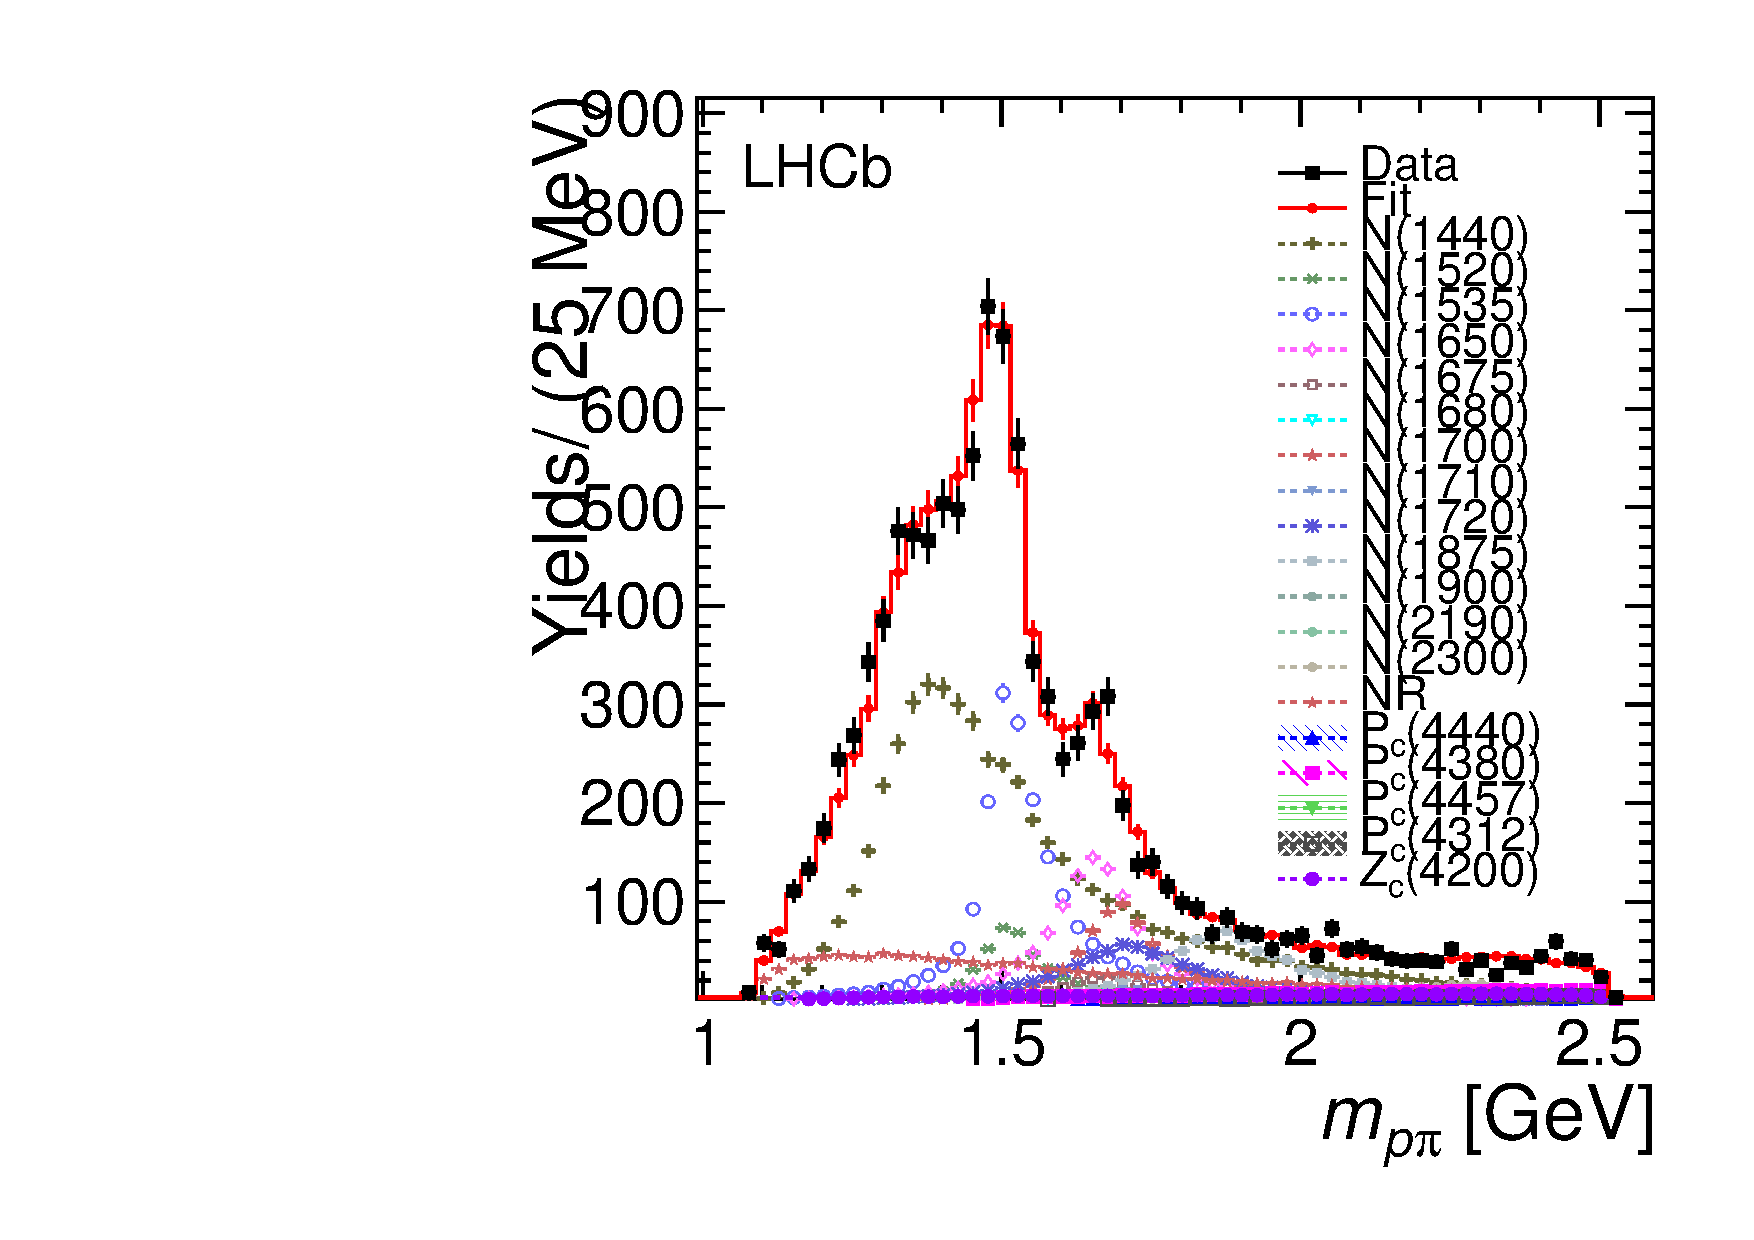
\includegraphics[width=0.4\textwidth]{Figures/04_Penta/05_fit_result/cor_plus3-plots/mppi_S}%
\put(-150,140) {\textrm{\small \bf Unofficial}}
\vskip -0.5cm
   \caption{Fit projections for $m_{\proton\pi}$ for the extended $N^*$ + 4$\ZP$ + $\ZC(4200)$ model. 
   The data are shown as solid (black) squares, 
   while the solid (red) line show the results of the fit. 
   The background is subtracted by sPlot technique. }\label{fig:fitpczc-ex}
\end{figure}

\begin{figure}[!tbp]
\begin{center}
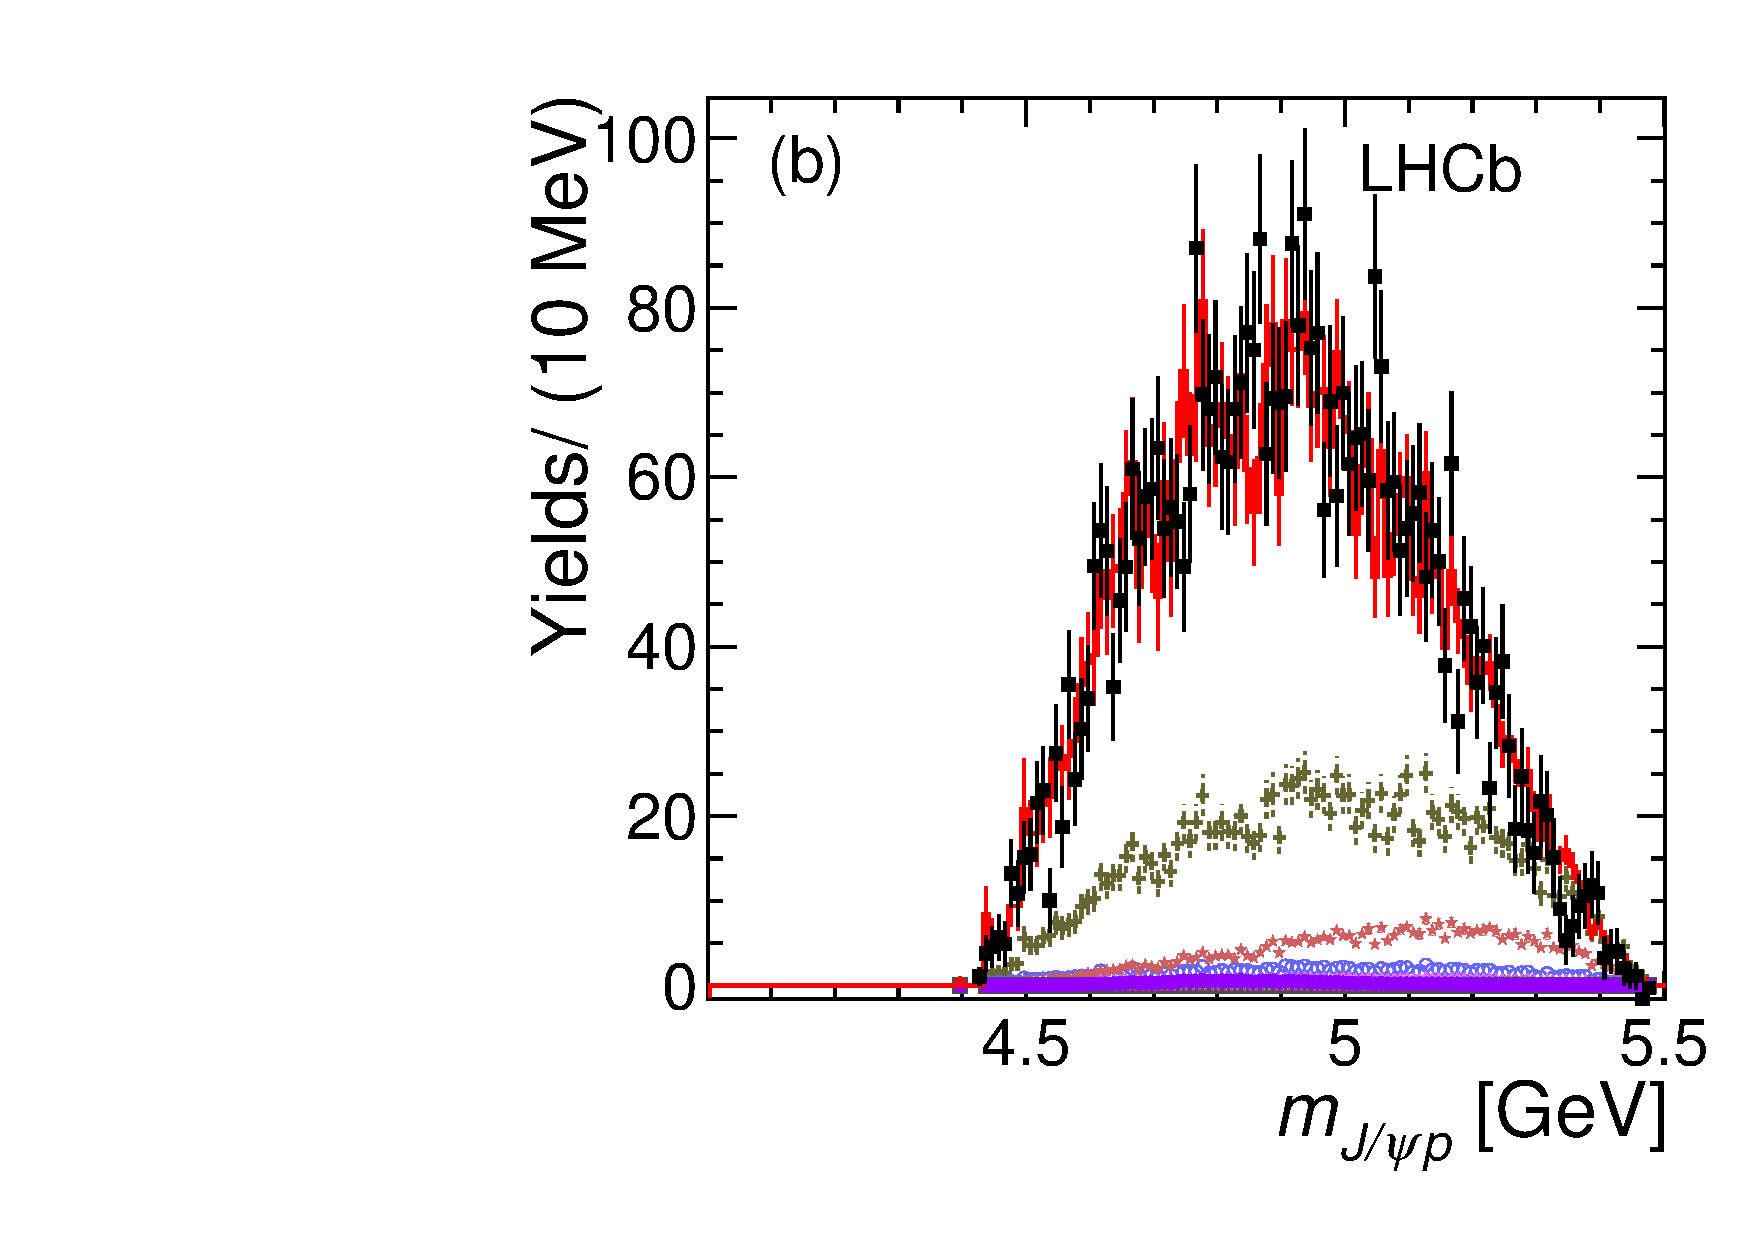
\includegraphics[width=0.4\textwidth]{Figures/04_Penta/05_fit_result/cor_plus3-plots/mjpsip1}%
\put(-60,140) {\textrm{\small \bf Unofficial}}
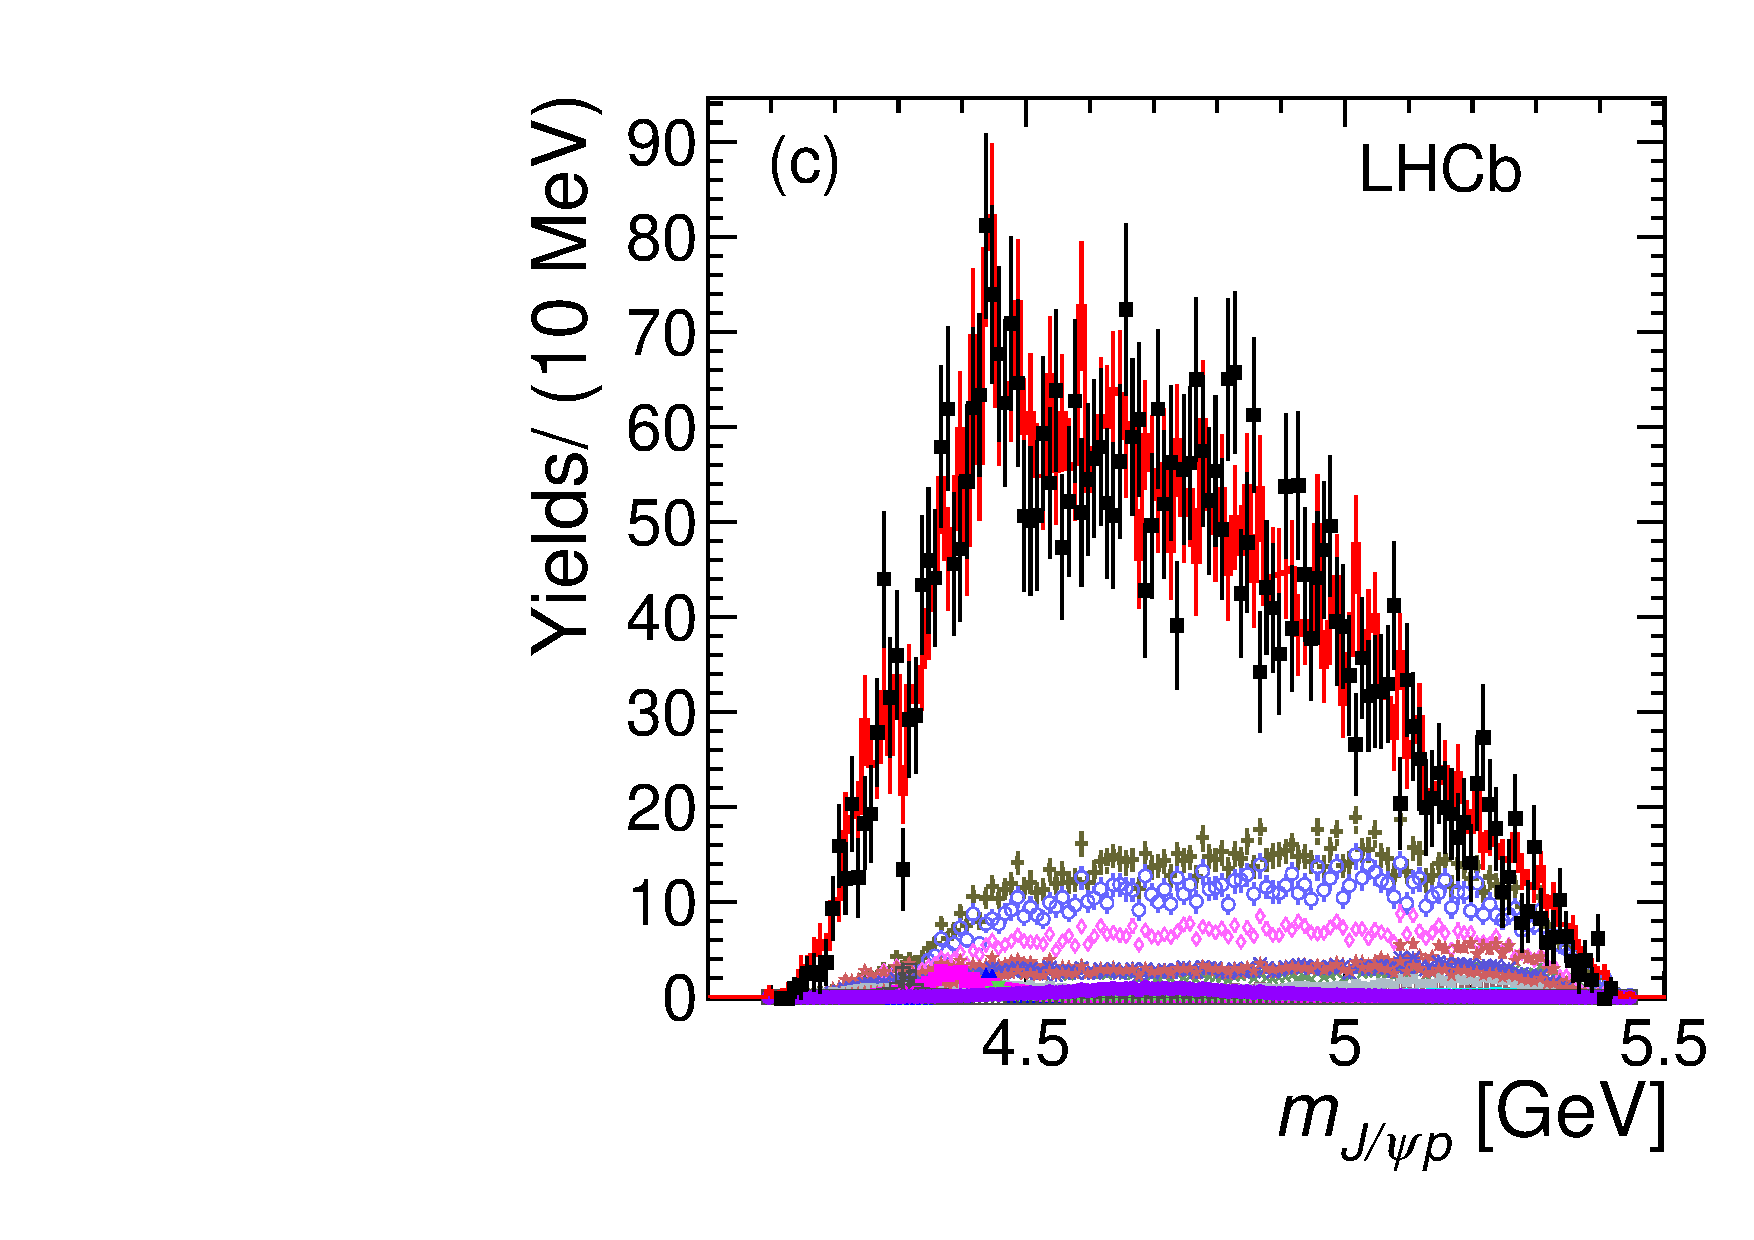
\includegraphics[width=0.4\textwidth]{Figures/04_Penta/05_fit_result/cor_plus3-plots/mjpsip2}
\put(-60,140) {\textrm{\small \bf Unofficial}}
\\
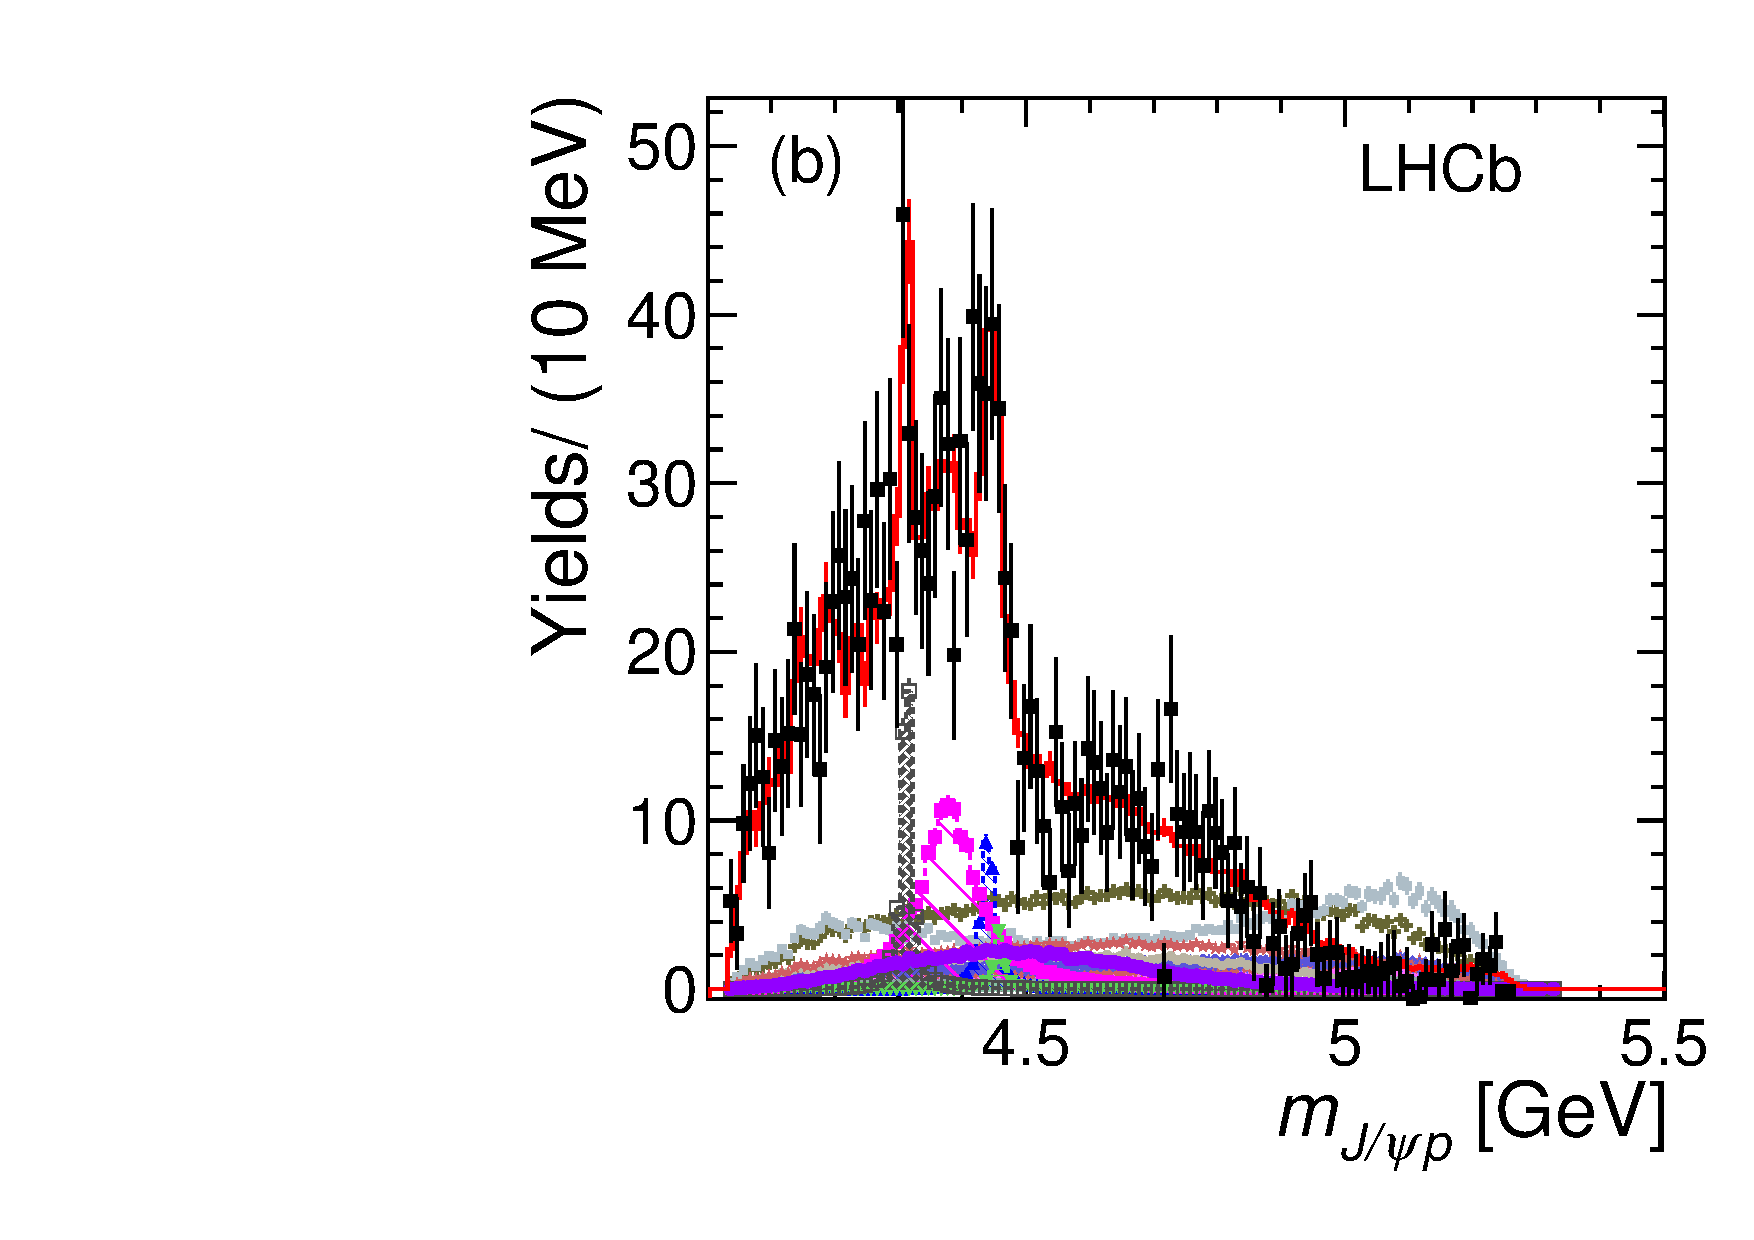
\includegraphics[width=0.4\textwidth]{Figures/04_Penta/05_fit_result/cor_plus3-plots/mjpsip3}
\put(-60,140) {\textrm{\small \bf Unofficial}}
\end{center}
\vskip -0.5cm
   \caption{$m_{\jpsi p}$ in various intervals of $m_{\proton\pi}$ for the extended $N^*+4\ZP+\ZC(4200)$ fit: 
   (a) no $m_{p\pi}$\gev cut, (b) $m_{p\pi}>1.80$\gev, and (c) $1.45<m_{p\pi}<1.80$\gev. 
   The data are shown as (black) squares, 
   while the (red) lines show the results of the fit.  
   The (green) dashed lines with open squares show the fit with $N^*$ only.}
\label{PcZc-mjpsip-bins-ex}
\end{figure}

\begin{figure}[!tbp]
\begin{center}
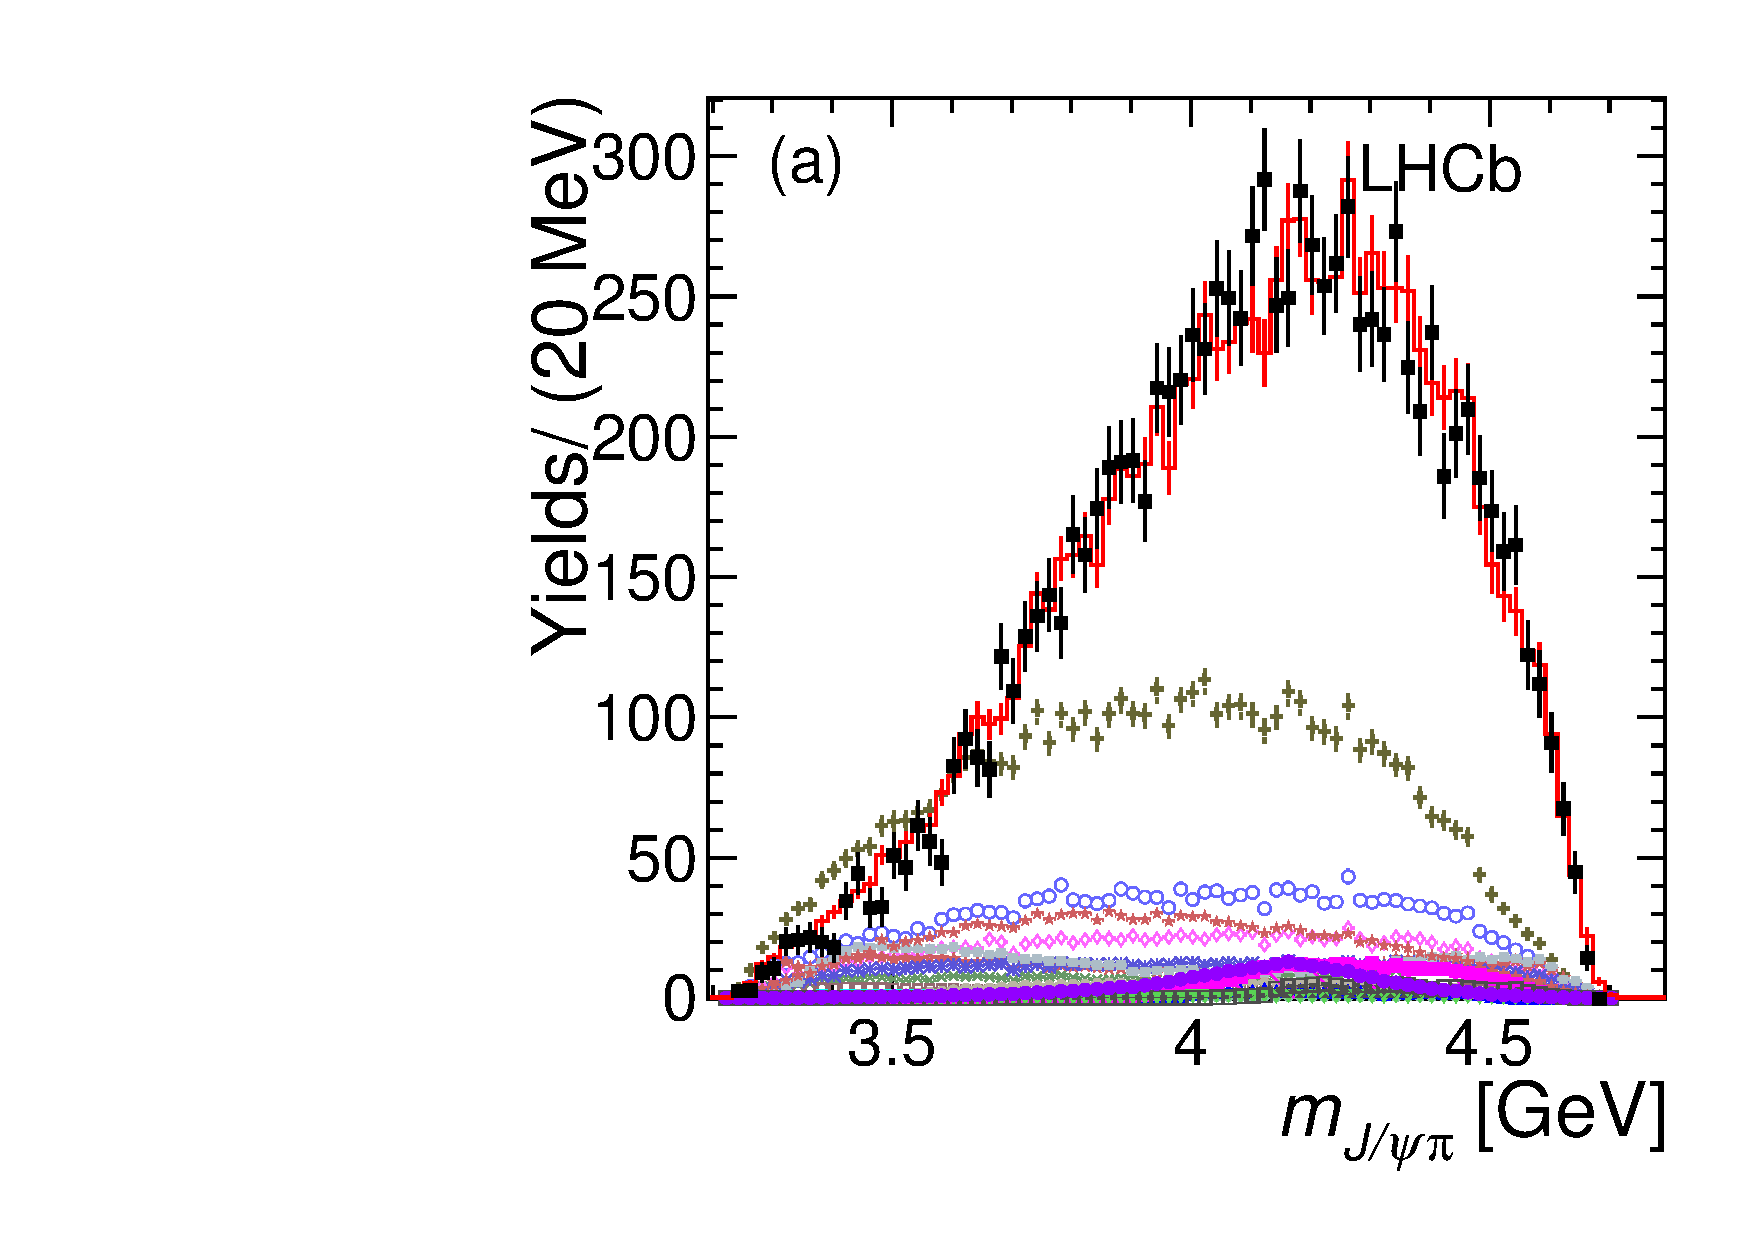
\includegraphics[width=0.4\textwidth]{Figures/04_Penta/05_fit_result/cor_plus3-plots/mjpsik0}%
\put(-150,140) {\textrm{\small \bf Unofficial}}
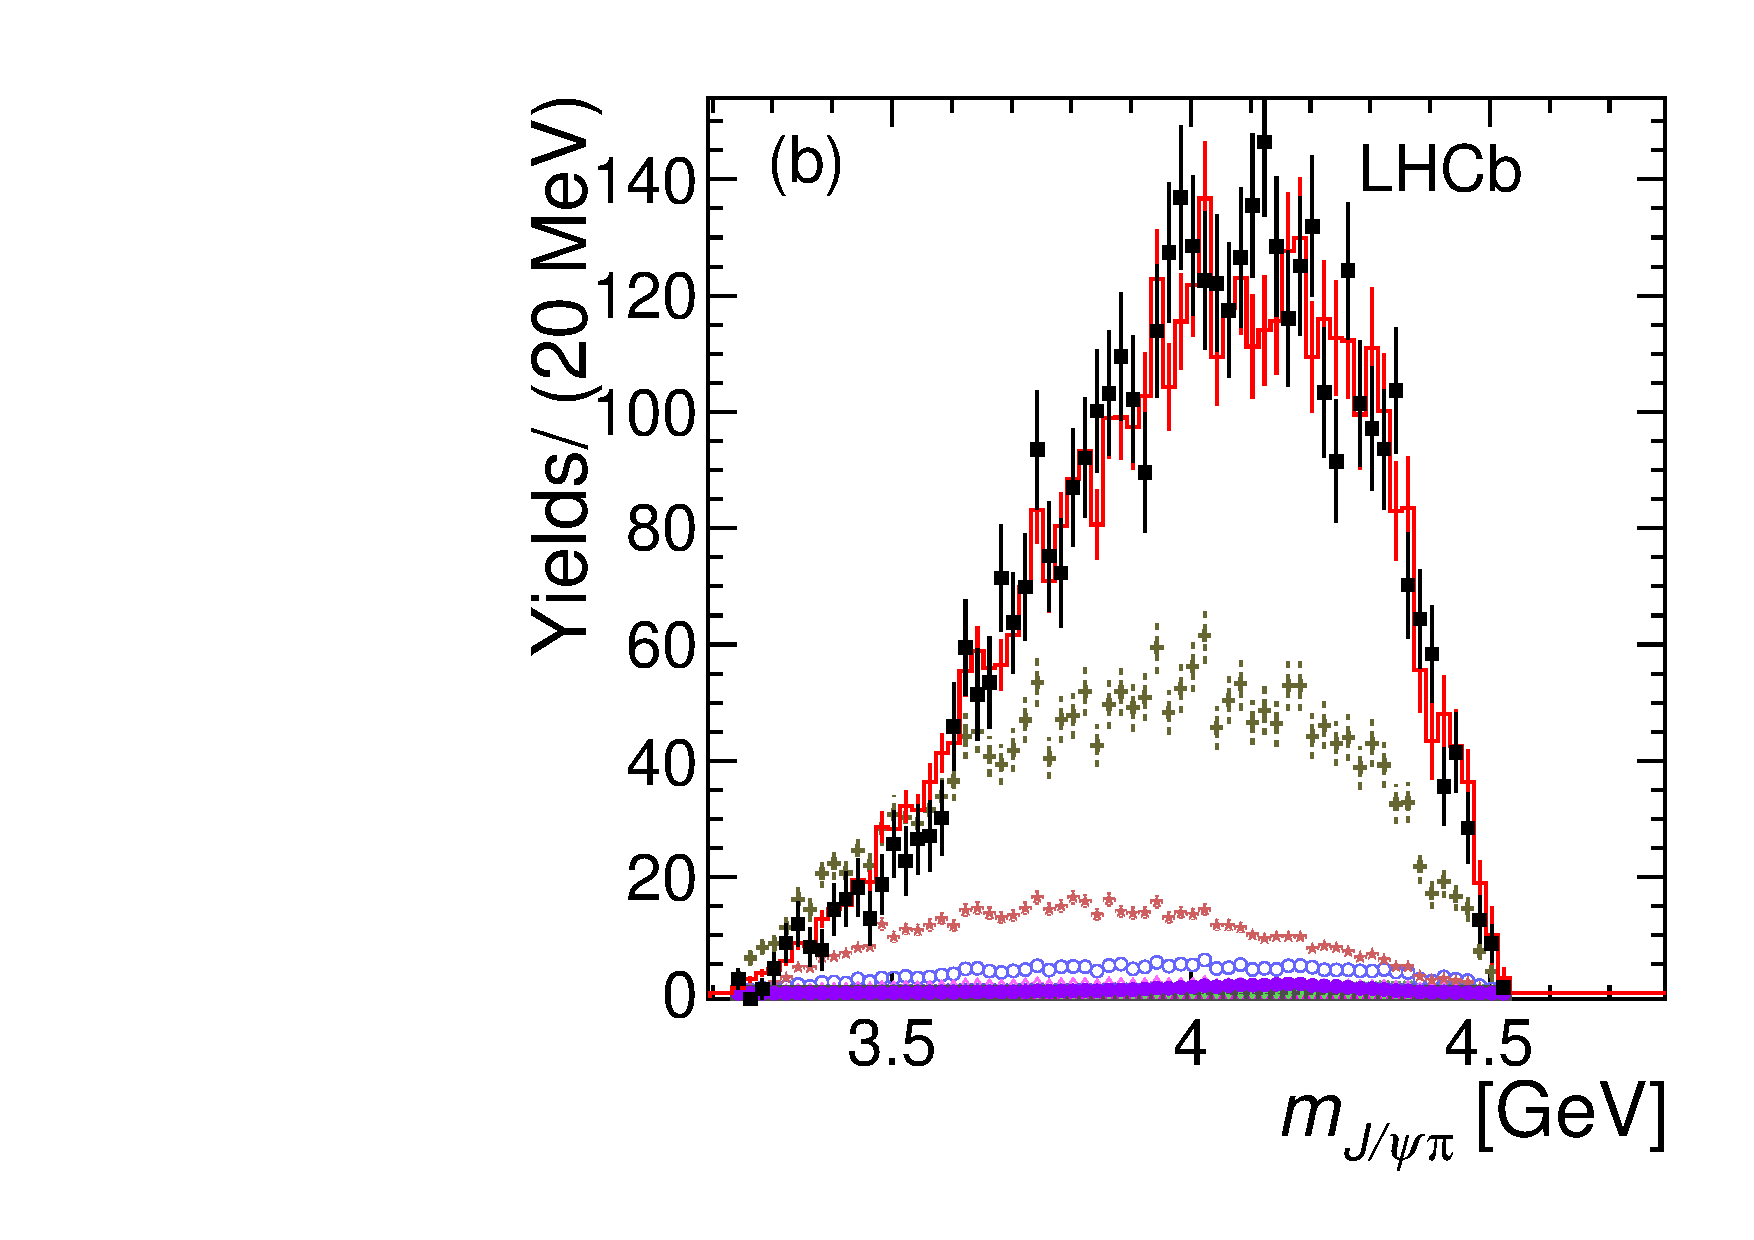
\includegraphics[width=0.4\textwidth]{Figures/04_Penta/05_fit_result/cor_plus3-plots/mjpsik1}
\put(-150,140) {\textrm{\small \bf Unofficial}} \\
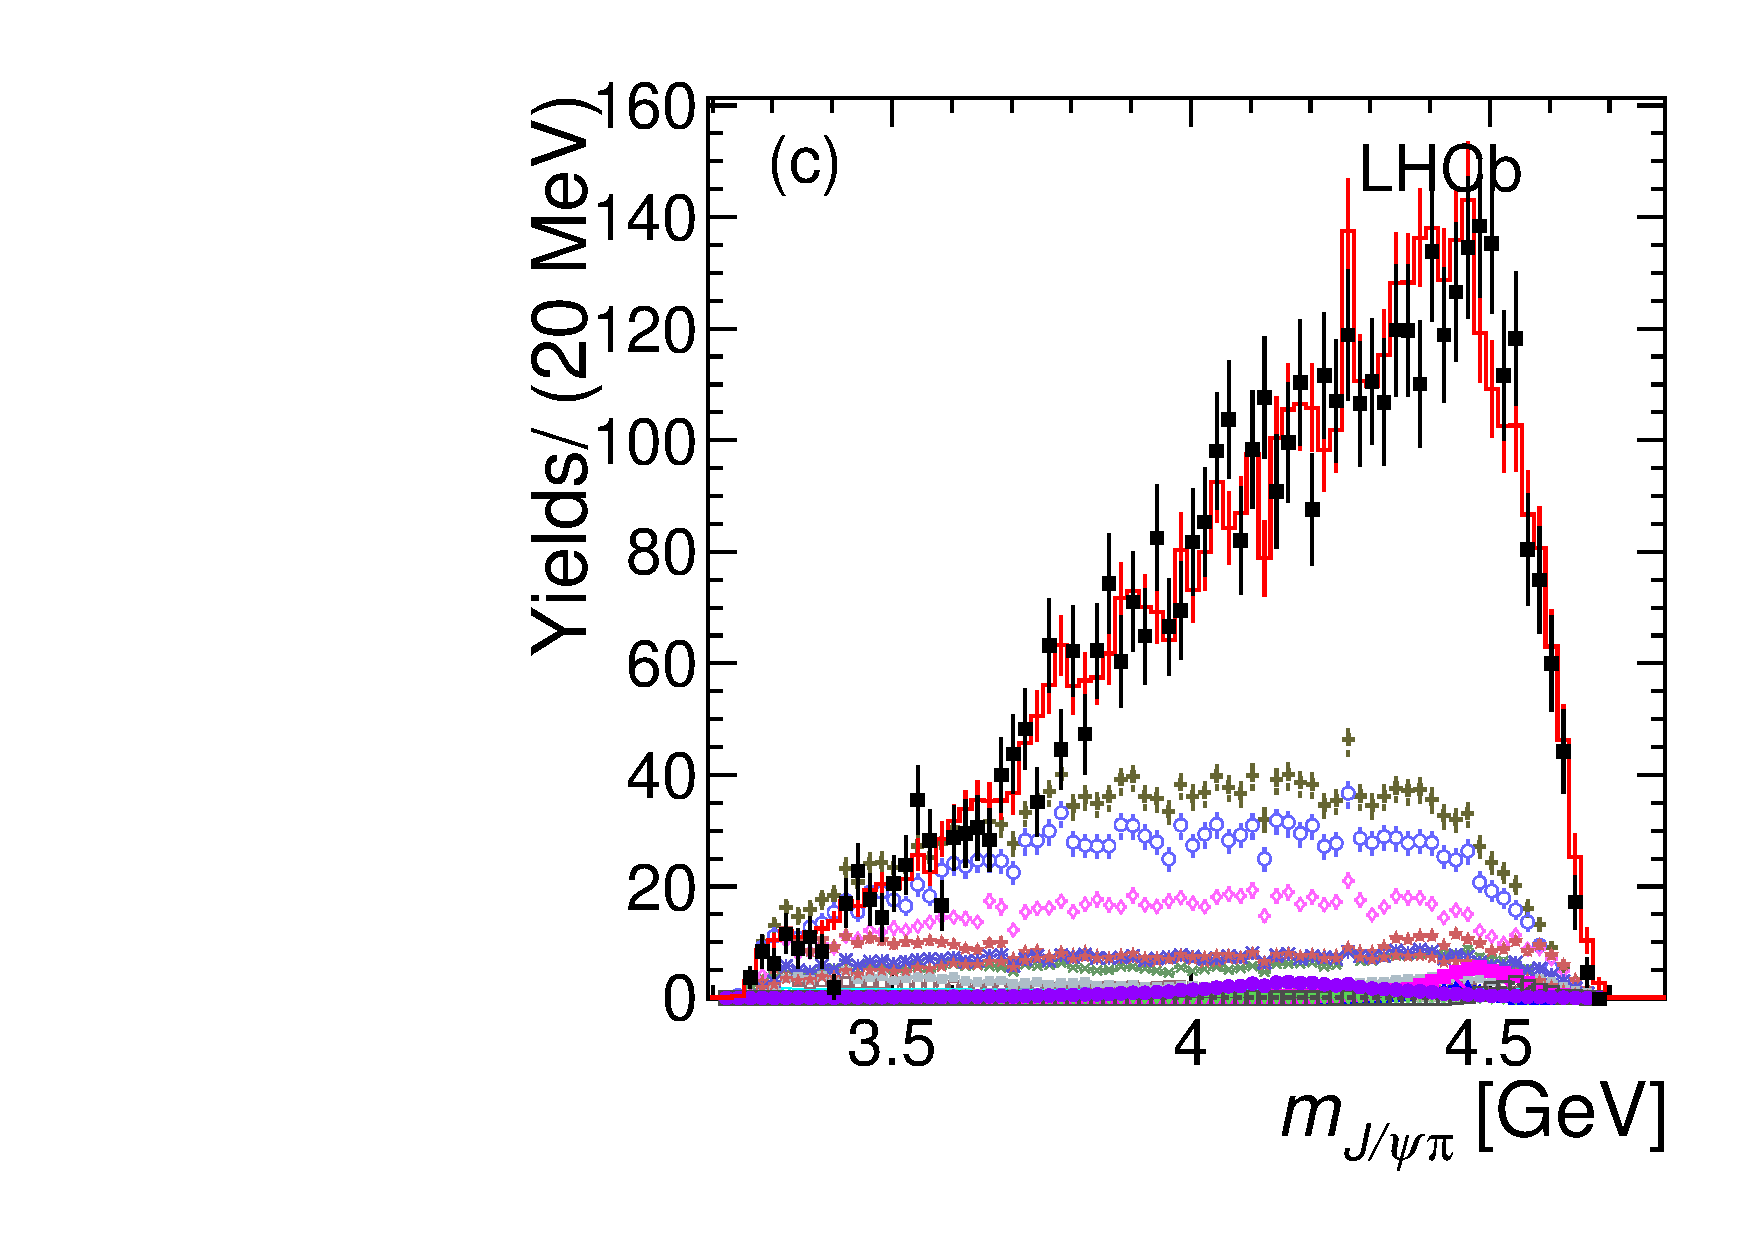
\includegraphics[width=0.4\textwidth]{Figures/04_Penta/05_fit_result/cor_plus3-plots/mjpsik2}%
\put(-150,140) {\textrm{\small \bf Unofficial}}
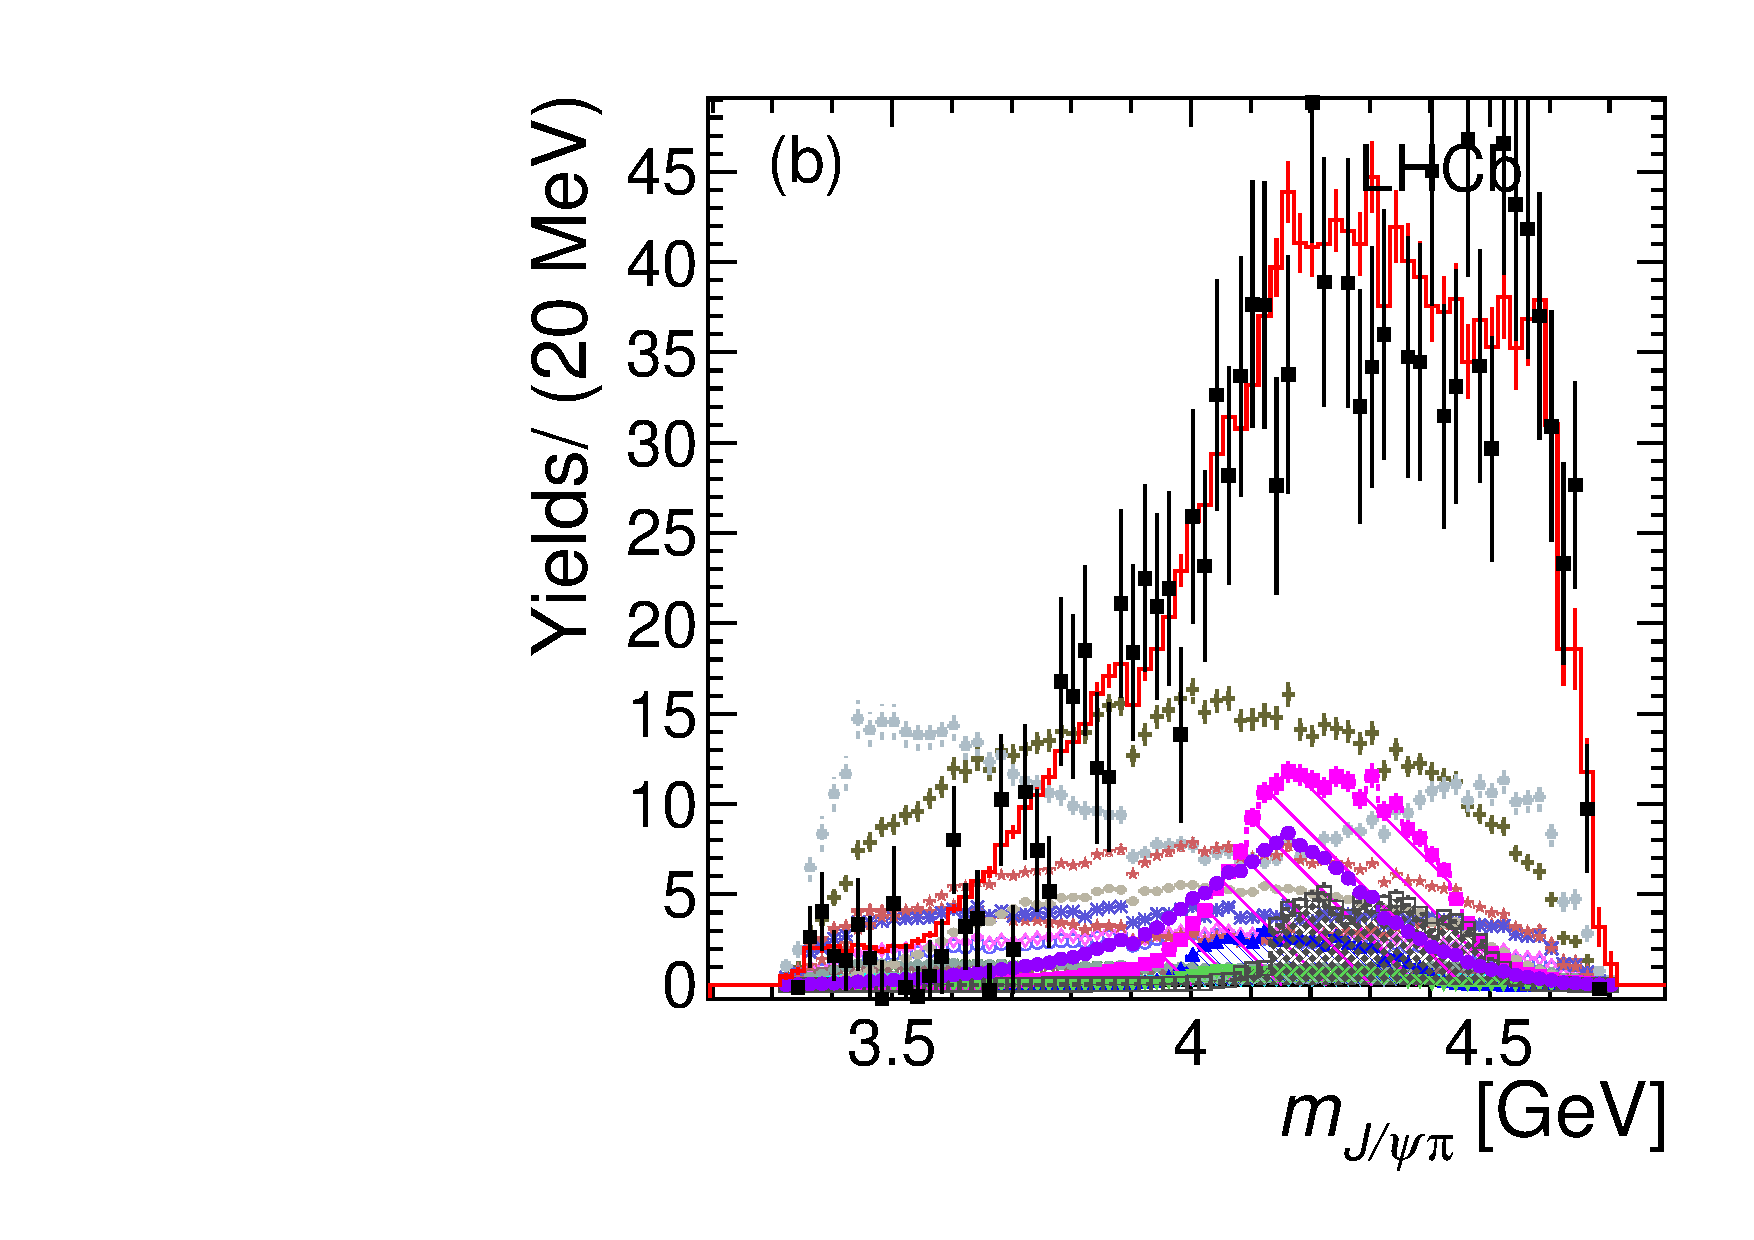
\includegraphics[width=0.4\textwidth]{Figures/04_Penta/05_fit_result/cor_plus3-plots/mjpsik3}
\put(-150,140) {\textrm{\small \bf Unofficial}}
\end{center}
\vskip -0.5cm
   \caption{$m_{\jpsi \pi}$ in various intervals of $m_{\proton\pi}$ for the extended $N^*+2\ZP+\ZC(4200)$ fit: 
   (a) all $m_{\proton\pi}$ (b) $m_{p\pi}<1.45$\gev, (c) $1.45<m_{p\pi}<1.80$\gev, and (d) $m_{p\pi}>1.80$\gev regions. 
   The data are shown as (black) squares, while the (red) lines show the results of the fit.}
\label{PcZc-mjpsipi-bins-ex}
\end{figure}



\begin{table}[htb]
\centering
\caption{ Extended model : $\Delta$(-2$\log(L)$). }
\label{tab:LL_extend}
\vspace{0.2cm}
\begin{tabular}{lc }
\hline\\[-2.5ex]
 State                                  &   $\Delta$(-2$\log(L)$)  \\ 
 \hline \\[-2.5ex]
 $N^*$                                  &   0(-13625.27)    \\
 $N^*+4P_c$                             &   -170.94    \\
 $N^*+4P_c-P_c(4440)$                   &   -158.97    \\
 $N^*+4P_c-P_c(4380)$                   &   -108.78    \\
 $N^*+4P_c-P_c(4457)$                   &   -163.50    \\
 $N^*+4P_c-P_c(4312)$                   &   -124.57    \\
 $N^*+4P_c-P_c(4440)-P_c(4457)$         &   -114.05    \\
 \hline
 $N^*+Z_c$                              &   -53.24    \\
 $N^*+Z_c+4P_c$                         &   -178.52    \\
 $N^*+Z_c+4P_c-P_c(4440)$               &   -167.55    \\
 $N^*+Z_c+4P_c-P_c(4380)$               &   -137.04    \\
 $N^*+Z_c+4P_c-P_c(4457)$               &   -171.06    \\
 $N^*+Z_c+4P_c-P_c(4312)$               &   -132.14    \\
 $N^*+Z_c+4P_c-P_c(4440)-P_c(4457)$     &   -130.18    \\
\hline
 $N^*+3P_c-P_c(4440)$                   &   -76.18    \\
 $N^*+3P_c-P_c(4457)$                   &   -95.89    \\
 $N^*+3P_c-P_c(4312)$                   &   -54.87    \\
 $N^*+3P_c-P_c(4440)-P_c(4457)$         &   -31.54    \\
\hline
 $N^*+Z_c+3P_c-P_c(4440)$               &   -113.40   \\
 $N^*+Z_c+3P_c-P_c(4457)$               &   -125.02   \\
 $N^*+Z_c+3P_c-P_c(4312)$               &   -89.43    \\
 $N^*+Z_c+3P_c-P_c(4440)-P_c(4457)$     &   -81.86    \\
 \hline
\end{tabular}
\end{table}

 \begin{table}[htb]
\centering
\caption{ Significance under various hypotheses with extended model. }
\label{tab:sig_extend}
\vspace{0.2cm}
\begin{tabular}{ l|c|c|c|c }
\hline\\[-2.5ex]
 State                   & $N^*+4P_c$   & $N^*+4P_c+Z_c$  & $N^*+3P_c$   & $N^*+3P_c+Z_c$  \\ 
 \hline \\[-2.5ex]
 $P_c(4440)$             & 3.0$\sigma$  & 2.9$\sigma$  & 5.3$\sigma$  & 4.5$\sigma$     \\
 $P_c(4380)$             & 7.6$\sigma$  & 6.1$\sigma$  & -            & -               \\
 $P_c(4457)$             & 2.2$\sigma$  & 2.3$\sigma$  & 3.3$\sigma$  & 3.1$\sigma$     \\
 $P_c(4312)$             & 6.5$\sigma$  & 6.5$\sigma$  & 7.0$\sigma$  & 6.6$\sigma$     \\
 $P_c(4440)+P_c(4457)$   & 6.8$\sigma$  & 6.1$\sigma$  & 8.0$\sigma$  & 6.6$\sigma$     \\
 $4P_c$                  & 11.9$\sigma$ & 9.9$\sigma$  & -            & -               \\
 $4P_c+Z_c$              & -            & 11.9$\sigma$ & -            & -     \\
 $Z_c$                   & -            & 2.3$\sigma$  & -            & 5.0$\sigma$     \\
\hline
\end{tabular}
\end{table}




%\begin{figure}[!tbp]
%\begin{center}
%\includegraphics[width=0.33\textwidth]{Ex/ang0}%
%\includegraphics[width=0.33\textwidth]{Ex/ang1}%
%\includegraphics[width=0.33\textwidth]{Ex/ang2}\\
%\includegraphics[width=0.33\textwidth]{Ex/ang3}%
%\includegraphics[width=0.33\textwidth]{Ex/ang4}
%\end{center}
%\vskip -0.5cm
%\caption{Various decay angular distributions for the $N^*+2\ZP+\ZC(4200)$ fit. The data are shown as (black) squares, while the (red) lines show the results of the fit.  See Fig.~\ref{fig:fitpczc-ex} for the legend. The angles are defined in the text.}
%\label{PcZc-angular-ex}
%\end{figure}
%
%\begin{figure}[!tbp]
%\begin{center}
%\includegraphics[width=0.33\textwidth]{Ex/ang0_3}%
%\includegraphics[width=0.33\textwidth]{Ex/ang1_3}%
%\includegraphics[width=0.33\textwidth]{Ex/ang2_3}\\
%\includegraphics[width=0.33\textwidth]{Ex/ang3_3}%
%\includegraphics[width=0.33\textwidth]{Ex/ang4_3}
%\end{center}
%\vskip -0.5cm
%\caption{Various decay angular distributions for the $N^*+2\ZP+\ZC(4200)$ fit in $\mppi>1.8$\gev. The data are shown as (black) squares, while the (red) lines show the results of the fit.  See Fig.~\ref{fig:fitpczc-ex} for the legend. The angles are defined in the text.}
%\label{PcZc-angular-3-ex}
%\end{figure}
%
%
%\begin{table}[tb]
%\centering
%\caption{$\Delta(\twolnL)$ in the fits with respect to the $N^*$ fit with the \EM under different $J^P$ assignments for ($\ZP(4380)$, $\ZP(4450)$), where the first two assignment are the best two preferences from the previous study.} 
%\label{tab:zcfit-ex}
%\begin{tabular}{clcccc}\hline
%Fit \# & Composition in fit & ($3/2^-$, $5/2^+$) & ($3/2^+$, $5/2^-$) & ($5/2^-$, $3/2^+$) & ($5/2^+$, $3/2^-$)  \\\hline
%1)	&	$N^*+\ZC$	&	31.5 	&	31.5 	&	31.5 	&	31.5 		\\	
%2)	&	$N^*+\ZP(4380)$	&	28.7 	&	24.5 	&	24.5 	&	29.9 		\\	
%3)	&	$N^*+\ZP(4450)$	&	18.8 	&	13.8 	&	16.7 	&	16.4 		\\	
%4)	&	$N^*+2\ZP$	&	39.1 	&	34.0 	&	37.5 	&	38.9 		\\	
%5)	&	$N^*+\ZC+\ZP(4380)$	&	38.2 	&	40.9 	&	31.6 	&	39.5 		\\	
%6)	&	$N^*+\ZC+\ZP(4450)$	&	32.5 	&	30.2 	&	32.3 	&	34.6 		\\	
%7)	&	$N^*+2\ZP+\ZC$	&	49.0 	&	50.6 	&	45.4 	&	52.8 		\\	\hline
%\end{tabular}
%\end{table}
%
%
%\begin{table}[tb]
%\centering
%\caption{$\Delta(\twolnL)/{\rm ndf}$ and significances under various hypotheses that either only $\ZC$ or only $2\ZP$ or both of them are present in the data using the smallest values among four $J^P$ combinations for the two $\ZP$ states. The ideal ndf are used for the significance calculations.} 
%\label{tab:zcsig-ex}
%\begin{tabular}{l|r|r|r}\hline
%State&$N^*+\ZC$	& $N^*+2\ZP$	& $N^*+2\ZP+\ZC$\\\hline
%$\ZC$&31.5/10=3.5$\sigma$&- &7.8/10=0.5$\sigma$\\
%$\ZP(4380)$&- &24.5/4=4.0$\sigma$&0.1/4=0$\sigma$ \\
%$\ZP(4450)$&- &9.1/4=1.8$\sigma$&9.7/4=2.0$\sigma$ 	\\
%$2\ZP$&-& 34.0/8=4.1$\sigma$ &13.9/8=1.7$\sigma$\\
%$2\ZP+\ZC$&-&-&45.4/18=3.6$\sigma$\\
%\hline
%\end{tabular}
%\end{table}
%
%





